\clearpage

\subsection{Scale factors for lepton efficiency}
\label{sec:scale-factors}

In Sections~\ref{sec:object-selection-electrons} and~\ref{sec:muon-selection}, the selection applied to electrons and muons was studied, and a choice was made regarding the identification working point used to draw conclusions about the identification efficiency of the leptons. However, relying solely on \gls{mc} can introduce systematic errors due to imperfections in modeling both the data and the detector response. Therefore, evaluating the level of consistency between data and \gls{mc} is important. To this end, the lepton efficiency is studied in data and \gls{mc}, where \emph{efficiency} refers to the fraction of produced leptons that are reconstructed, selected and identified as such:
\begin{equation}
\varepsilon_{\ell} = \frac{N_{\ell}(\text{reconstructed, selected, and identified})}{N_{\ell}(\mathrm{produced})}
\end{equation}
In \gls{mc}, the number of produced leptons is simply the number of generated leptons. However, in data, the efficiency must be measured in another way. Once the efficiency has been measured both in simulation and data, a correction factor called the \gls{sf} can be applied as weights to the simulation to correct for discrepancies that may arise. Scale factors are defined as the ratio between the efficiency in data and the efficiency in simulation:

\begin{equation}
\mathrm{SF}_{\ell}=\frac{\varepsilon_{\ell}^{\mathrm{Data}}}{\varepsilon_{\ell}^{\mathrm{MC}}}.
\end{equation}

The \glspl{sf} are applied as weights for each lepton that passes the object selection in the event. The scale factors for loose-ID electrons in the relevant \pt range have been centrally measured by the corresponding CMS working group and are applied to the selected electrons. Scale factors for needed (Medium) ID muons with $\pt\geq 2\GeV$ were computed centrally by the Muon \gls{pog}. However, as mentioned in~\cite{muon-id-sf-2016,muon-id-sf-2016-pres}, the scale factors were computed by requiring $\DR > 0.5$, which excludes the key phase space that drives the sensitivity, as discussed in Section~\ref{sec:lepton-dr}. Therefore, it is necessary to evaluate any potential $\DR$ dependence. To this end, the efficiency in different $\DR$ regions is extracted  from an analysis of $\JPsi$ decays.

To measure the lepton efficiency in data, a tag and probe method is employed. This method often makes use of a known mass resonance such as \PZ, \JPsi or \PGU to select particles using very loose selection criteria on one of the objects (the probe). The efficiency of applying one or more election criteria is then computed as the fraction of probe particles that satisfy this criteria. The mass resonance results in the formation of a peaking structure in the invariant mass of the tag and probe system, from which the number of total and passing probe particles can be extracted via a sideband fit. To measure the efficiency, muon/track pairs are selected with an invariant mass near the \JPsi mass. The muon is labeled as the `tag' and the track as a `probe'. The tag muon is selected with a medium selection, listed in Table~\ref{tab:tag-probe-def}, resulting in high certainty that the object corresponds to a real produced muon. The probe (inner tracker track) corresponds to a very inclusive object, with no selection corresponding to the muon ID applied to it, a loose selection but constrained to be consistent with a decay of a \JPsi. The background contribution, originating from random tracks as well as fake muons, is removed by a simultaneous fit of a smoothly falling background and the shape of the \JPsi. The probes are then subjected to the requirement that the track be matched within $\DR<0.01$ of an analysis muon. The efficiency in question is written as:

\begin{equation}
\varepsilon_{\mu} = \frac{N_{\mu}^\text{Matched}}{N_{t}}.
\end{equation}

The selection applied on the objects corresponding to the numerator and denominator are summarized in Table~\ref{tab:tag-probe-def}. This study was conducted for the year 2016. The 2016 samples listed in Section~\ref{sec:sm-mc} are used for \gls{mc}. To ensure the independence of the tagged muon from the triggered object, a single electron trigger is used for data. The luminosity of the corresponding data set is measured to be 36.02\fbinv using the BRIL Work Suite~\cite{bril}. The following trigger paths are utilized:
\begin{itemize}
\item \texttt{HLT\_Ele27\_WPTight\_Gsf\_v*},
\item \texttt{HLT\_Ele27\_eta2p1\_WPLoose\_Gsf\_v*},
\item \texttt{HLT\_Ele32\_WPTight\_Gsf\_v*},
\item \texttt{HLT\_Ele35\_WPTight\_Gsf\_v*}.
\end{itemize}
An offline loose ID electron with $\pt>27\GeV$ is then selected. The requirements to select a tag and probe pair are defined in Table~\ref{tab:tag-probe-def}.

\begin{table}[!htb]
	\centering
	
		\caption{\label{tab:tag-probe-def}Selection criteria for tags and probes}
		%\vspace{1mm}
			\begin{tabular}{l|l} \hline
			Tag & Probe \\ \hline
			Medium ID muon & isolated track\\
			$\pt \geq 5\GeV$ & $2\leq\pt\leq 20\GeV$  ($ \pt\geq 3 \GeV $ for barrel) \\
			$\abs{\eta}<2.4$ & opposite-sign, in invariant mass window $[2.5,3.5]\GeV$ \\ \hline
			\end{tabular}
\end{table}

A fit is performed in an invariant mass window around the \JPsi peak of $[2.5,3.5]\GeV$. The signal PDF is modelled using a double-sided Crystal Ball function, and the continuum is modelled with a 6th order polynomial. The fit is repeated twice, once for the denominator based on probe tracks, and once for the numerator using those tracks that have been matched to Medium ID muons. The $\DR$ range has been split into three, and the $\abs{\eta}$ of the muons has been divided into barrel ($\abs{\eta}<1.2$) and endcaps ($1.2<\abs{\eta}<2.4$). Fits to the \gls{mc} are shown in Figure~\ref{fig:tb-barrel-simulation} for the barrel and Figure~\ref{fig:tb-endcaps-simulation} for the endcaps. Fits to the data are shown in Figure~\ref{fig:tb-barrel-data} for the barrel and Figure~\ref{fig:tb-endcaps-data} for the endcaps.

\begin{figure}[!htbp]
\centering
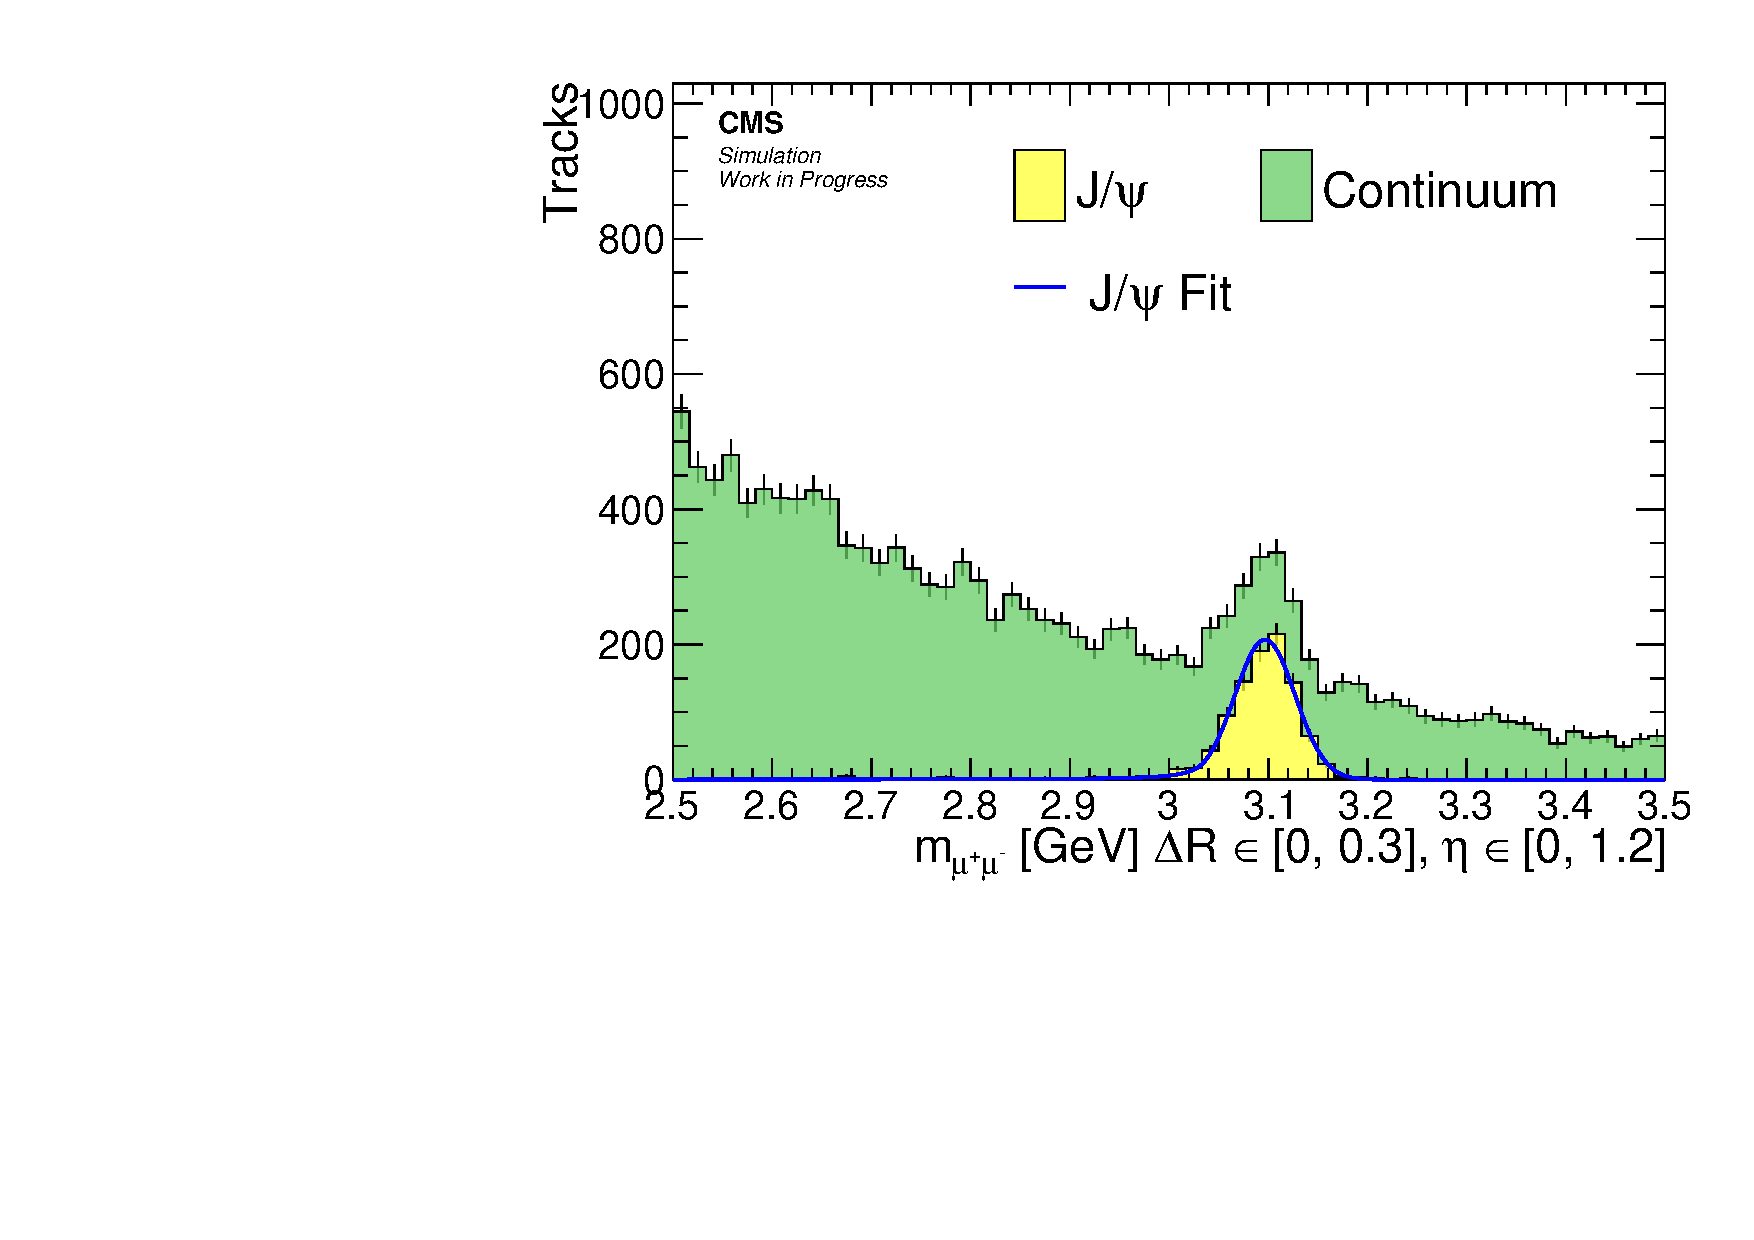
\includegraphics[width=0.32\linewidth]{plots/jpsi_muons_fit_bg_delta_r_single_electron/none_invMass_0_0.3_0_1.2.pdf} \,
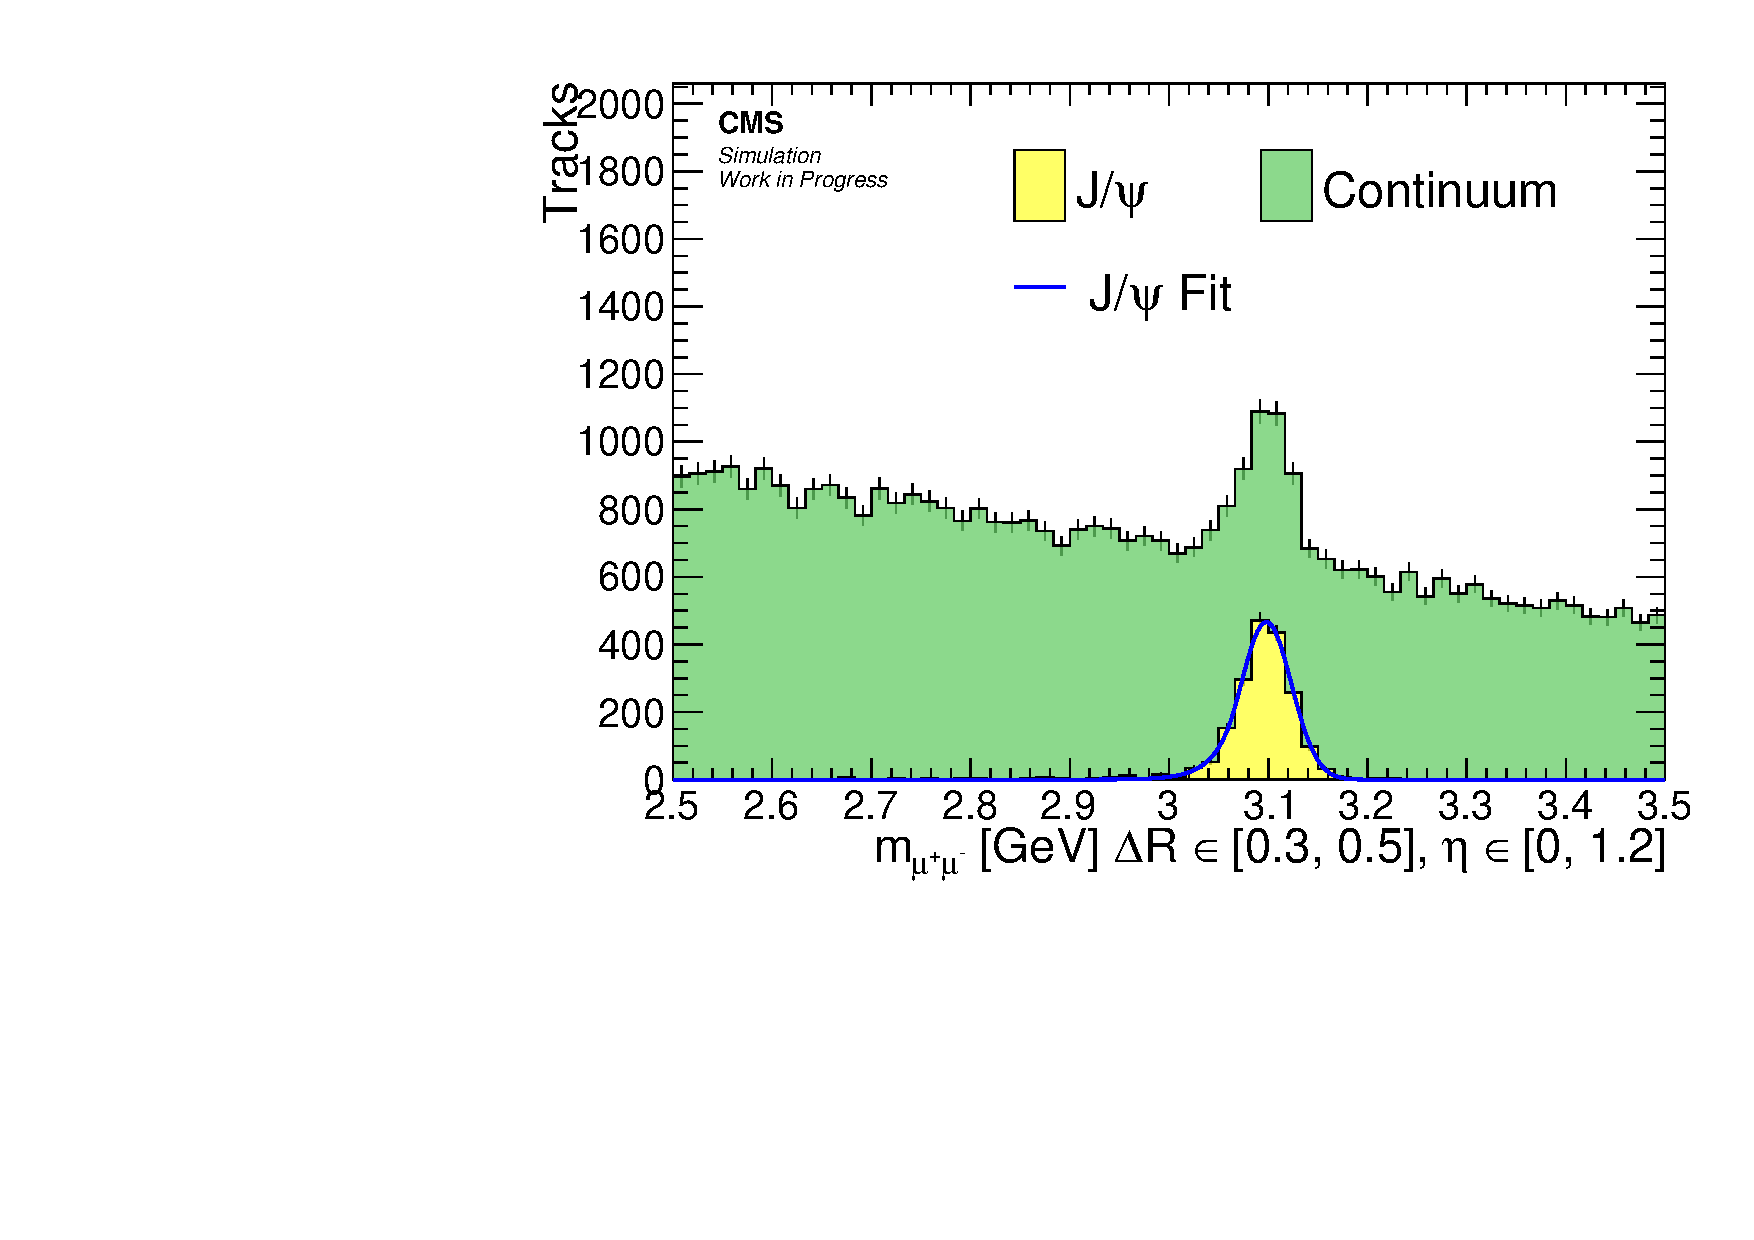
\includegraphics[width=0.32\linewidth]{plots/jpsi_muons_fit_bg_delta_r_single_electron/none_invMass_0.3_0.5_0_1.2.pdf}  \,
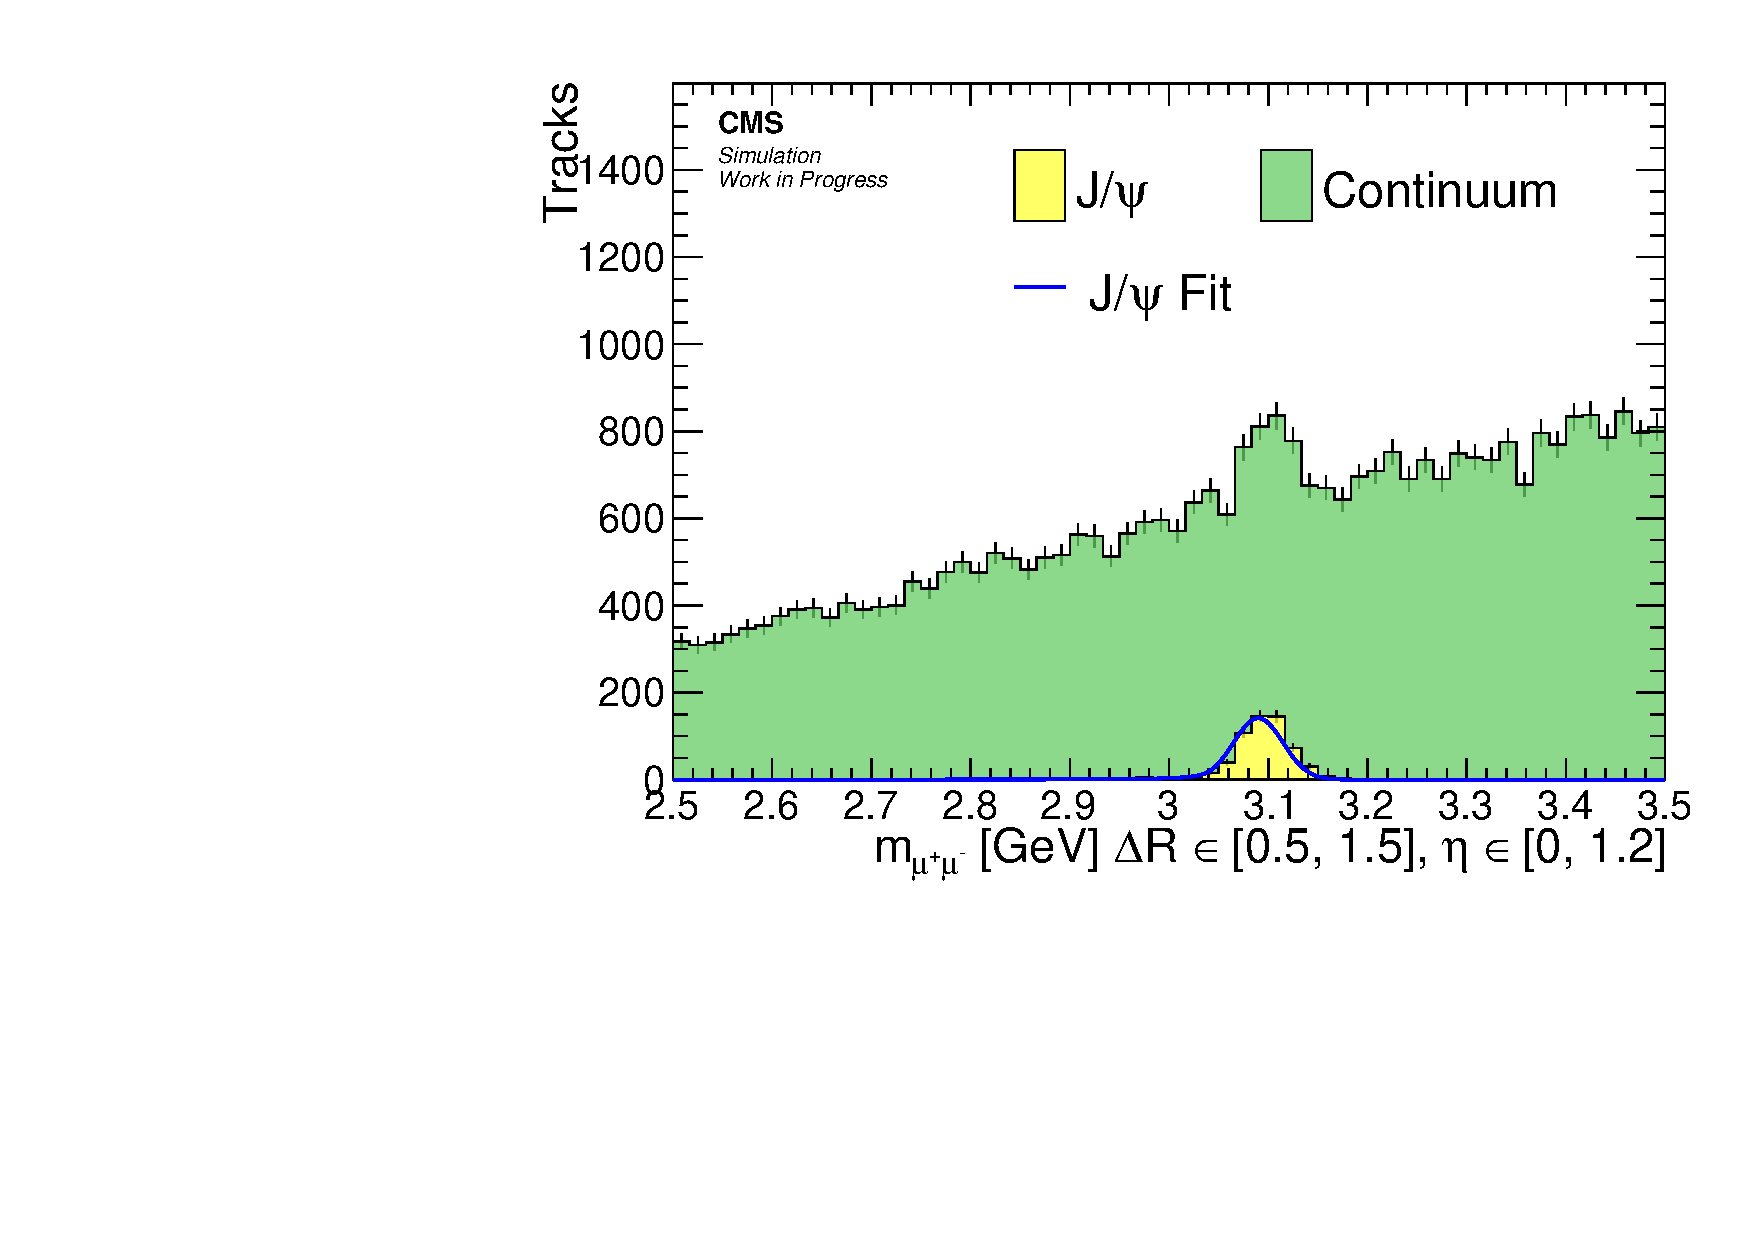
\includegraphics[width=0.32\linewidth]{plots/jpsi_muons_fit_bg_delta_r_single_electron/none_invMass_0.5_1.5_0_1.2.pdf} \\
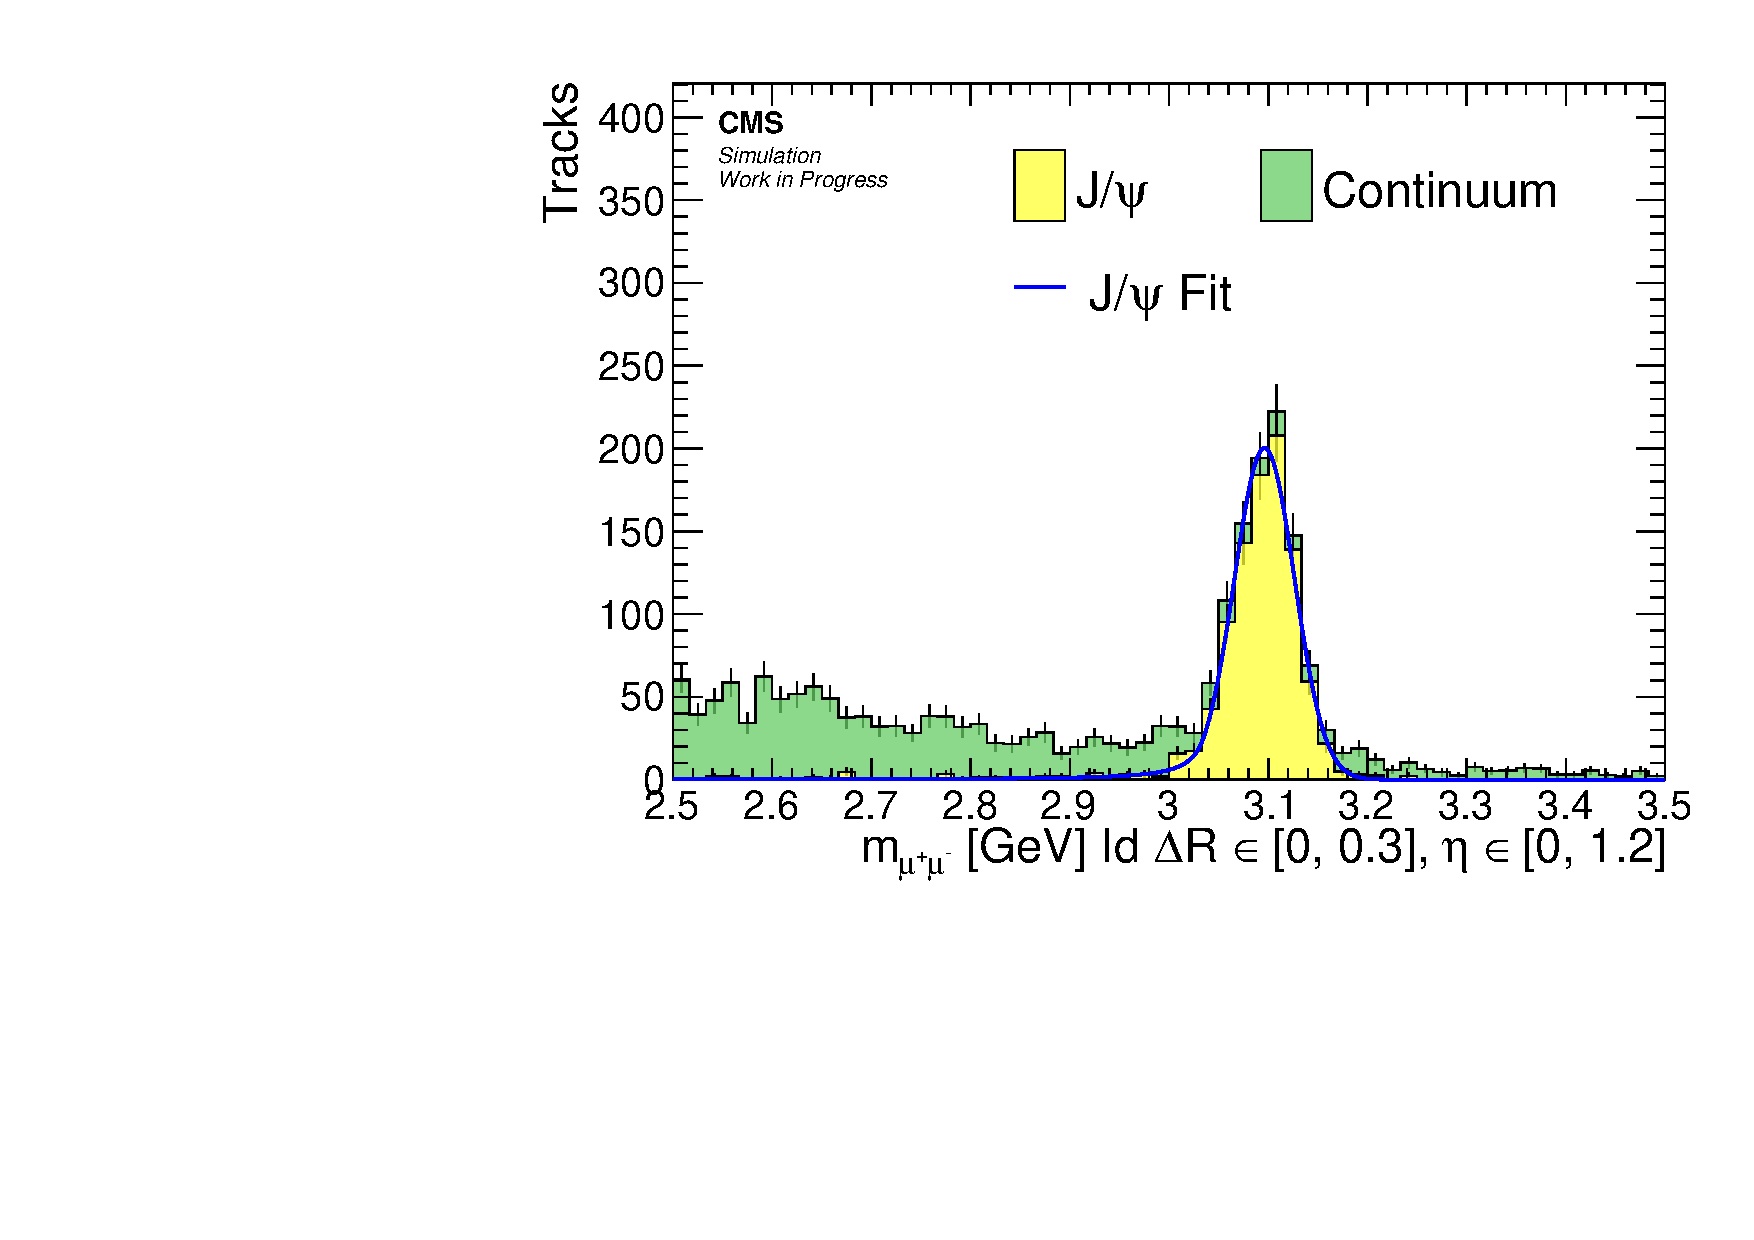
\includegraphics[width=0.32\linewidth]{plots/jpsi_muons_fit_bg_delta_r_single_electron/none_id_invMass_0_0.3_0_1.2.pdf} \,
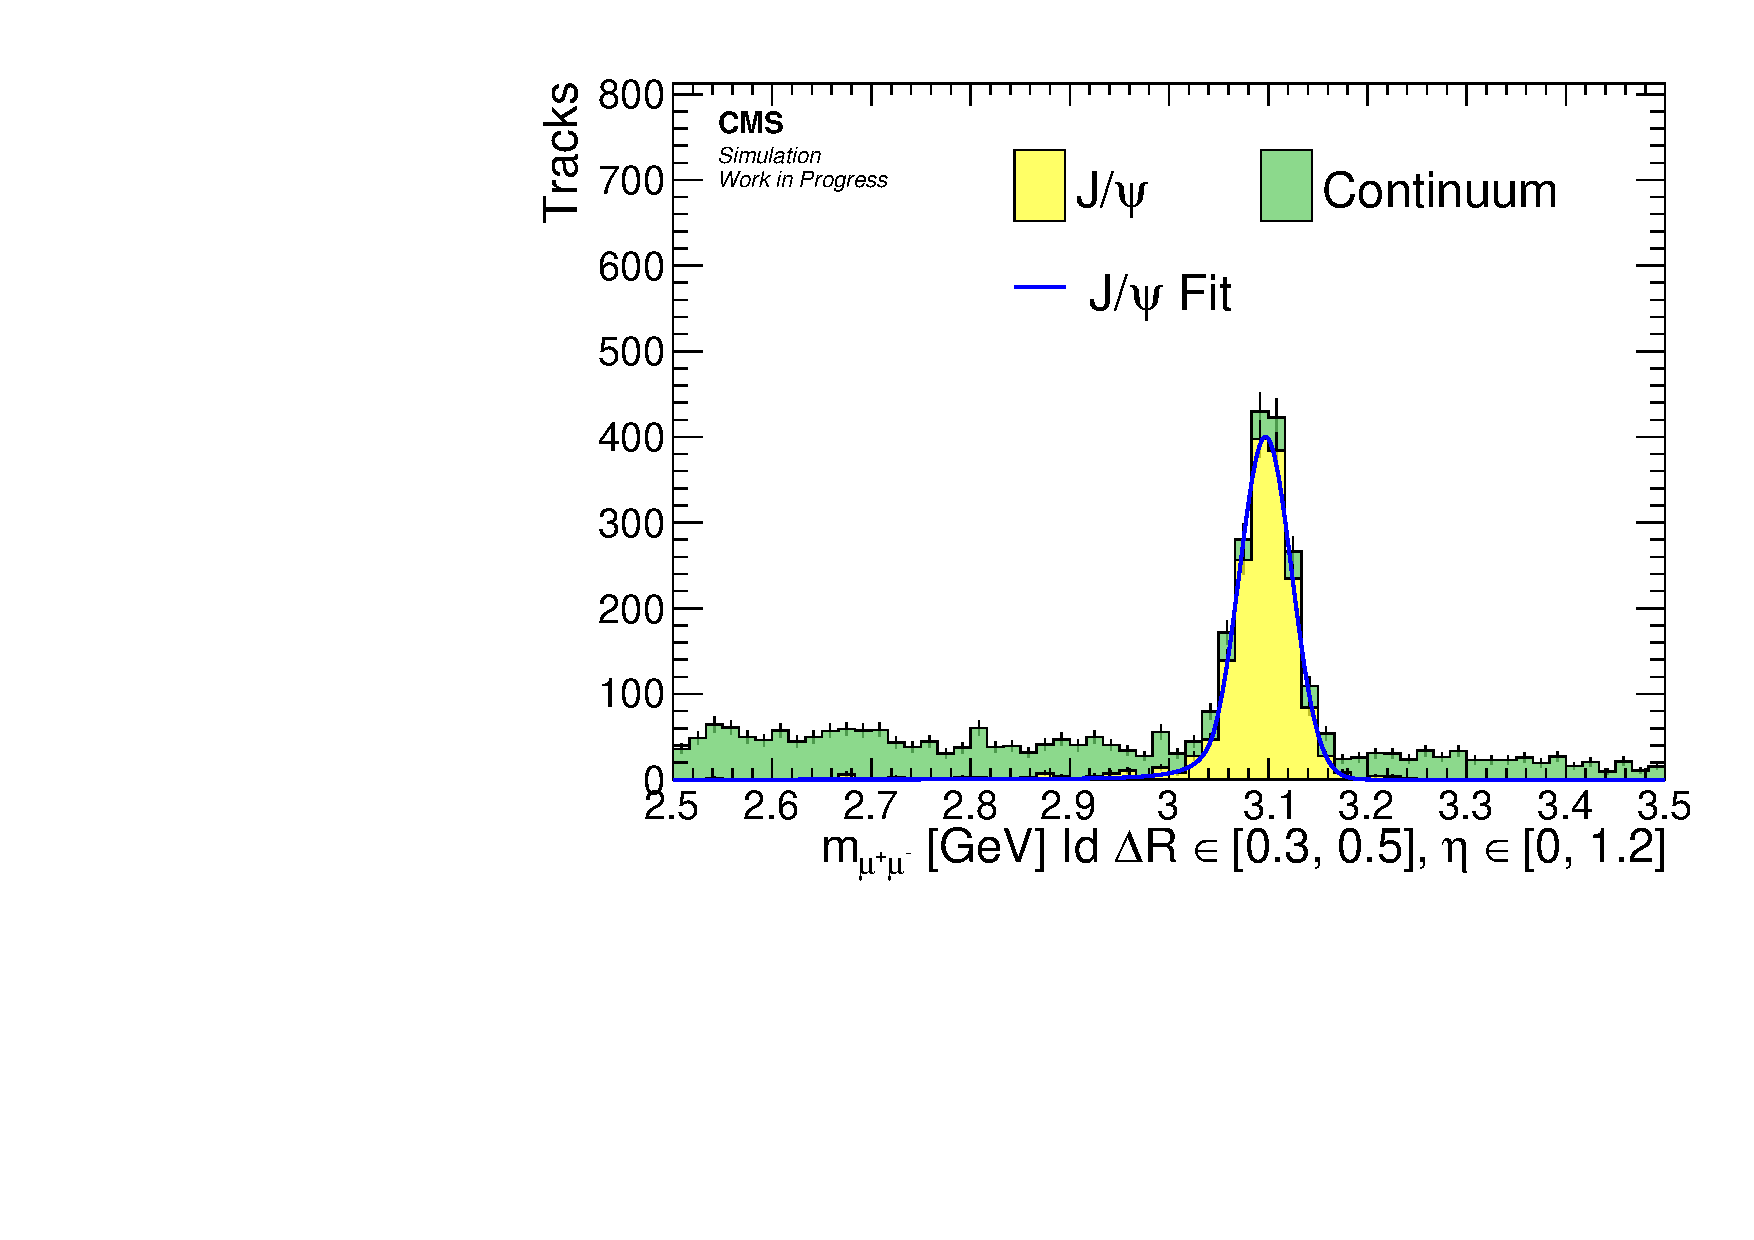
\includegraphics[width=0.32\linewidth]{plots/jpsi_muons_fit_bg_delta_r_single_electron/none_id_invMass_0.3_0.5_0_1.2.pdf}  \,
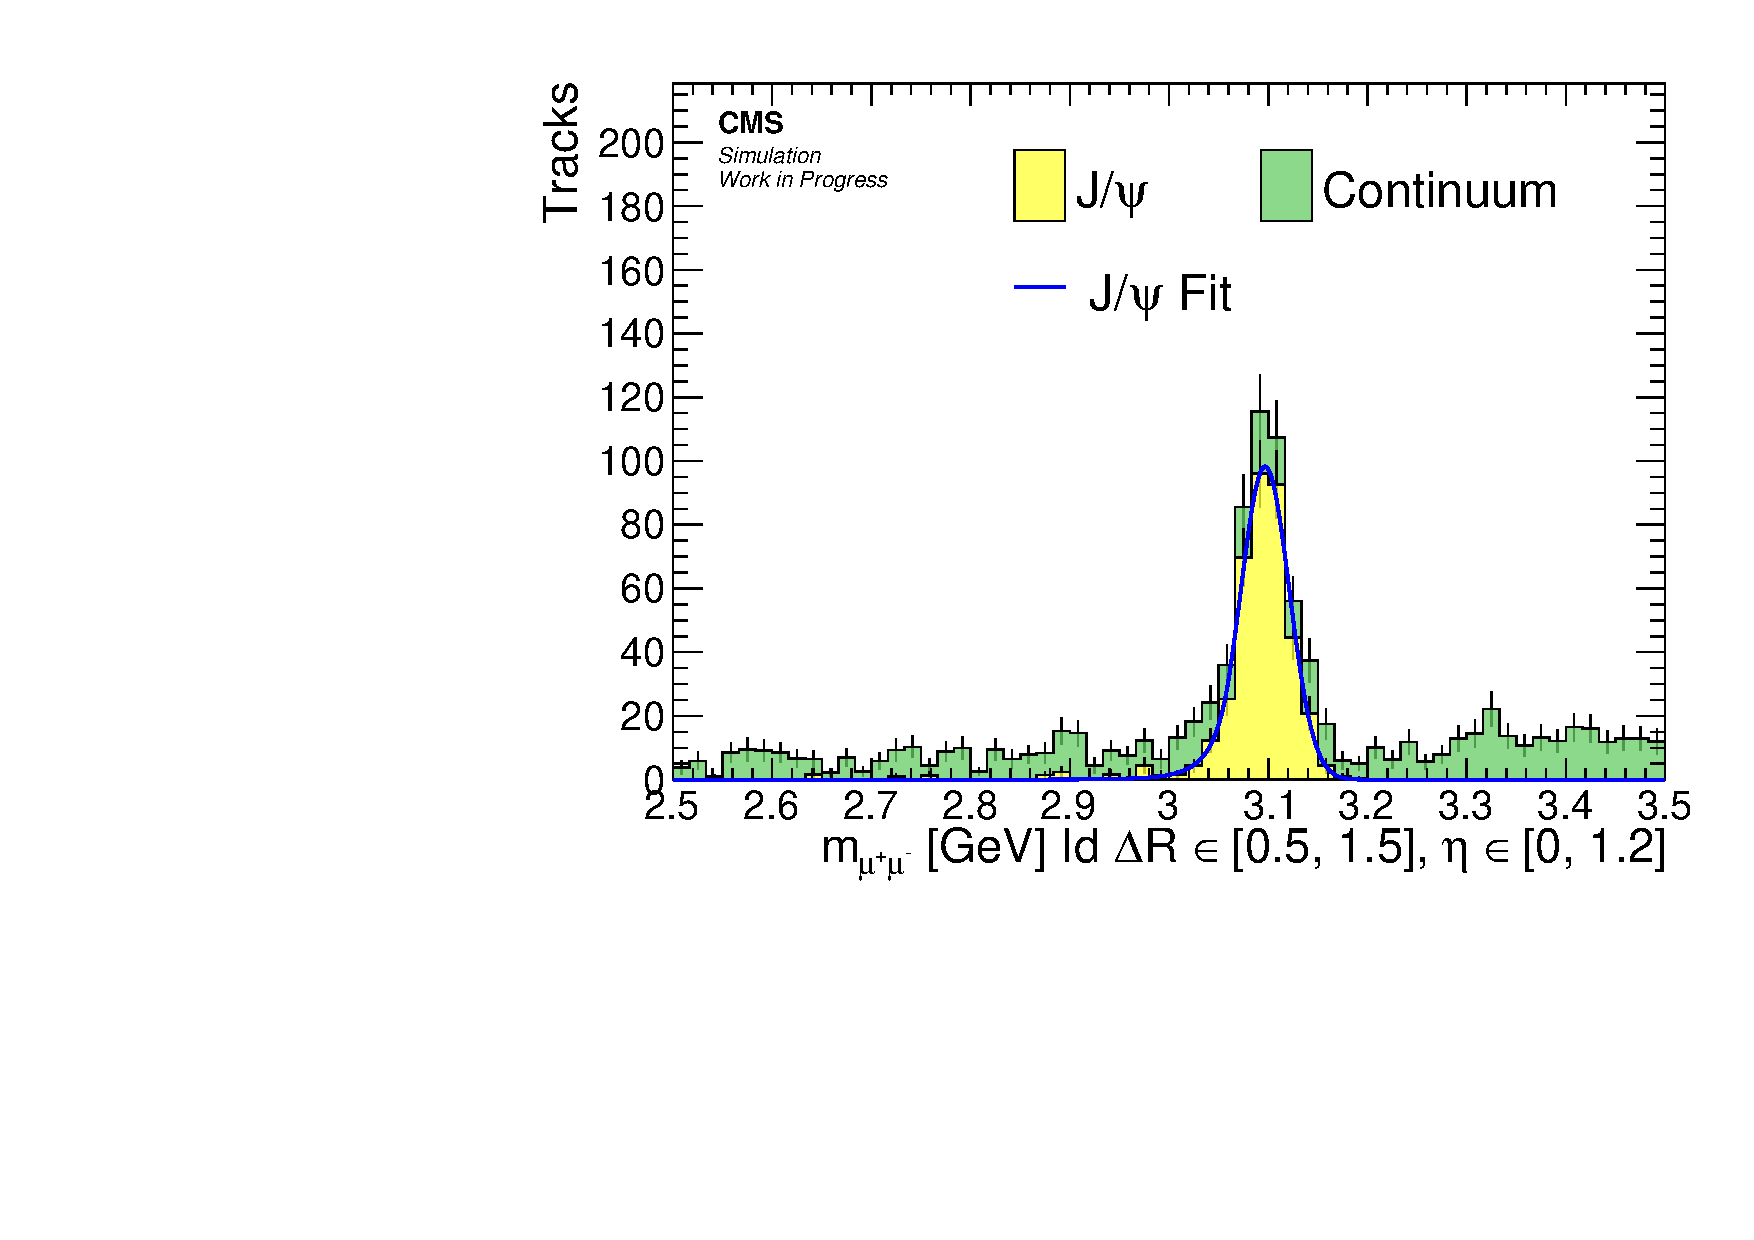
\includegraphics[width=0.32\linewidth]{plots/jpsi_muons_fit_bg_delta_r_single_electron/none_id_invMass_0.5_1.5_0_1.2.pdf} \\
\caption[Simluation barrel muons fits]{Fits to the tag and probe invariant mass for muons in the barrel region based on MC. Results are shown for denominator (top) and numerator (bottom) for $0<\DR<0.3$  (left), $0.3<\DR<0.5$ (center), $0.5<\DR<1.5$ (right).}
\label{fig:tb-barrel-simulation}
\end{figure}

\begin{figure}[!htbp]
\centering
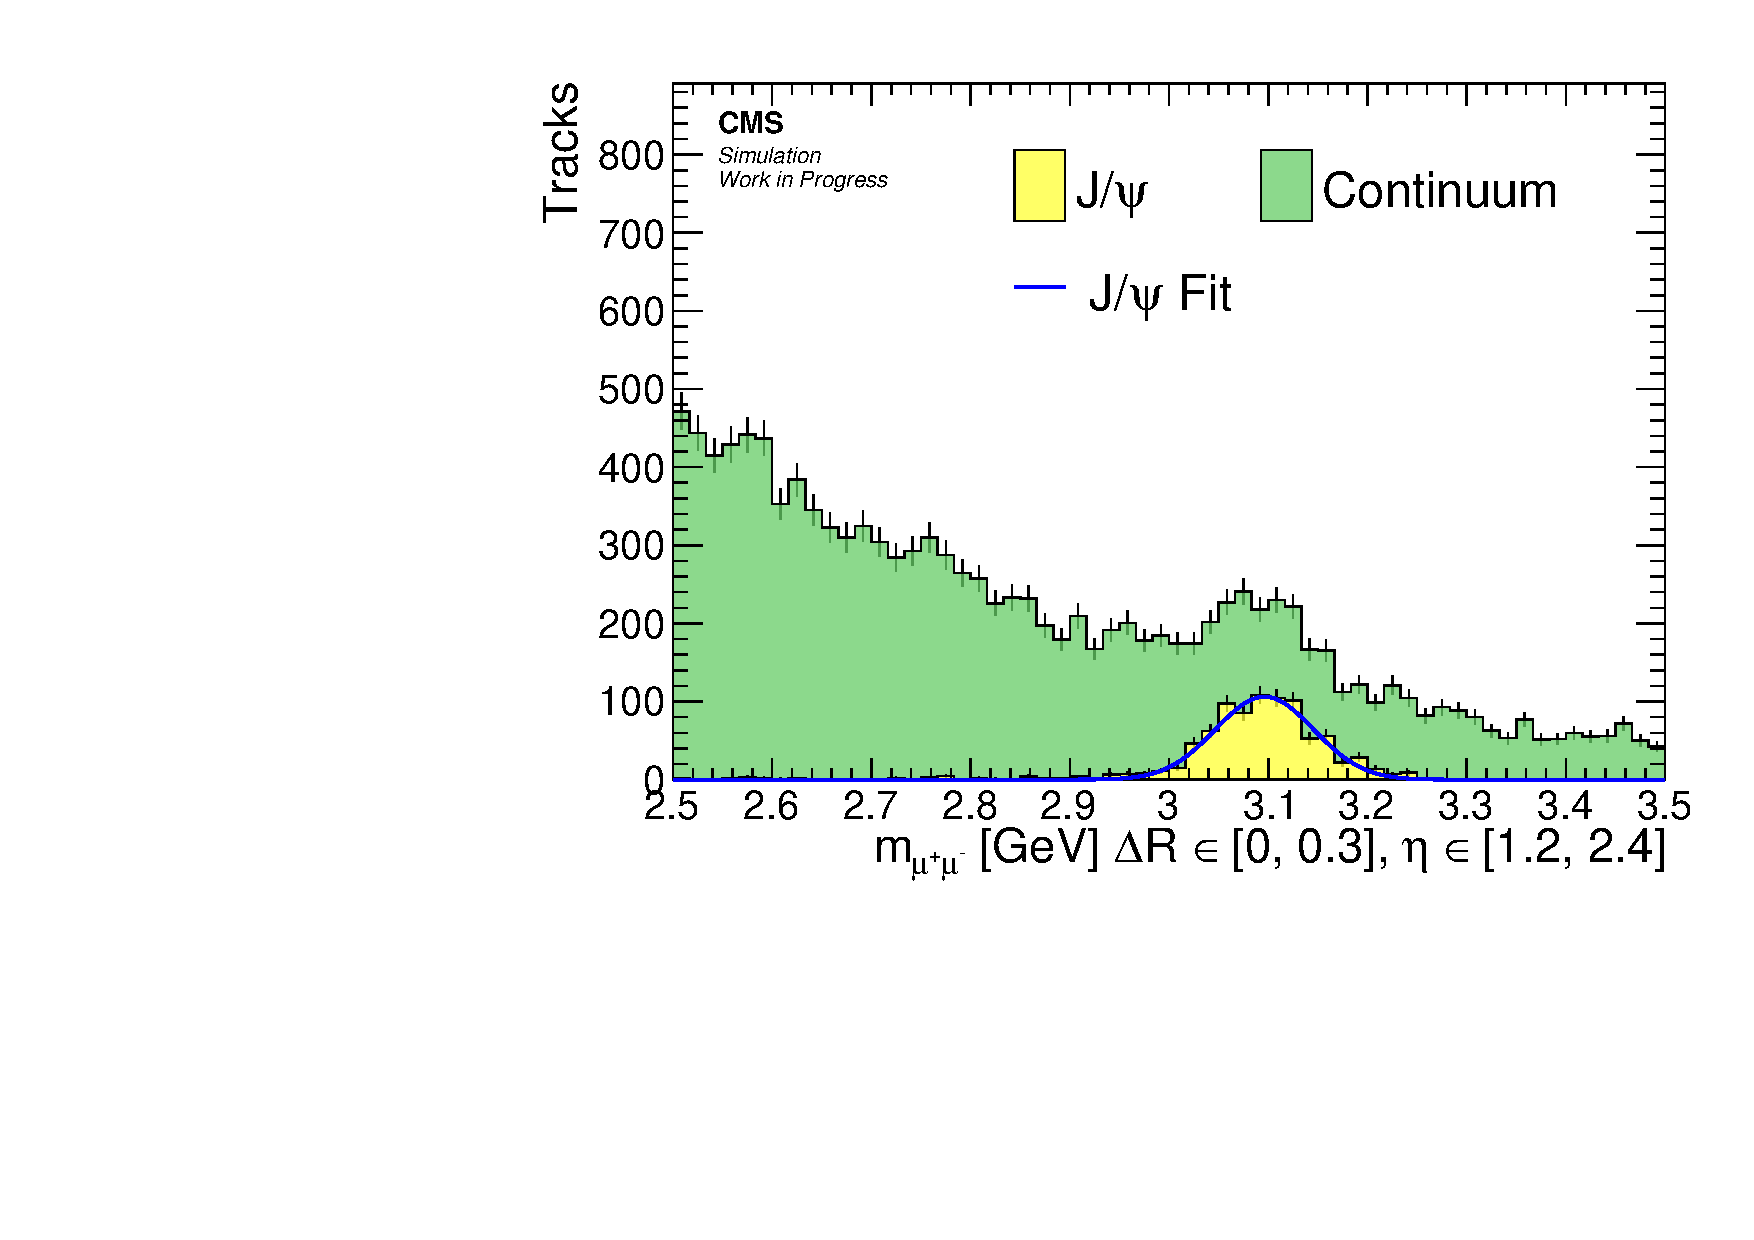
\includegraphics[width=0.32\linewidth]{plots/jpsi_muons_fit_bg_delta_r_single_electron/none_invMass_0_0.3_1.2_2.4.pdf} \,
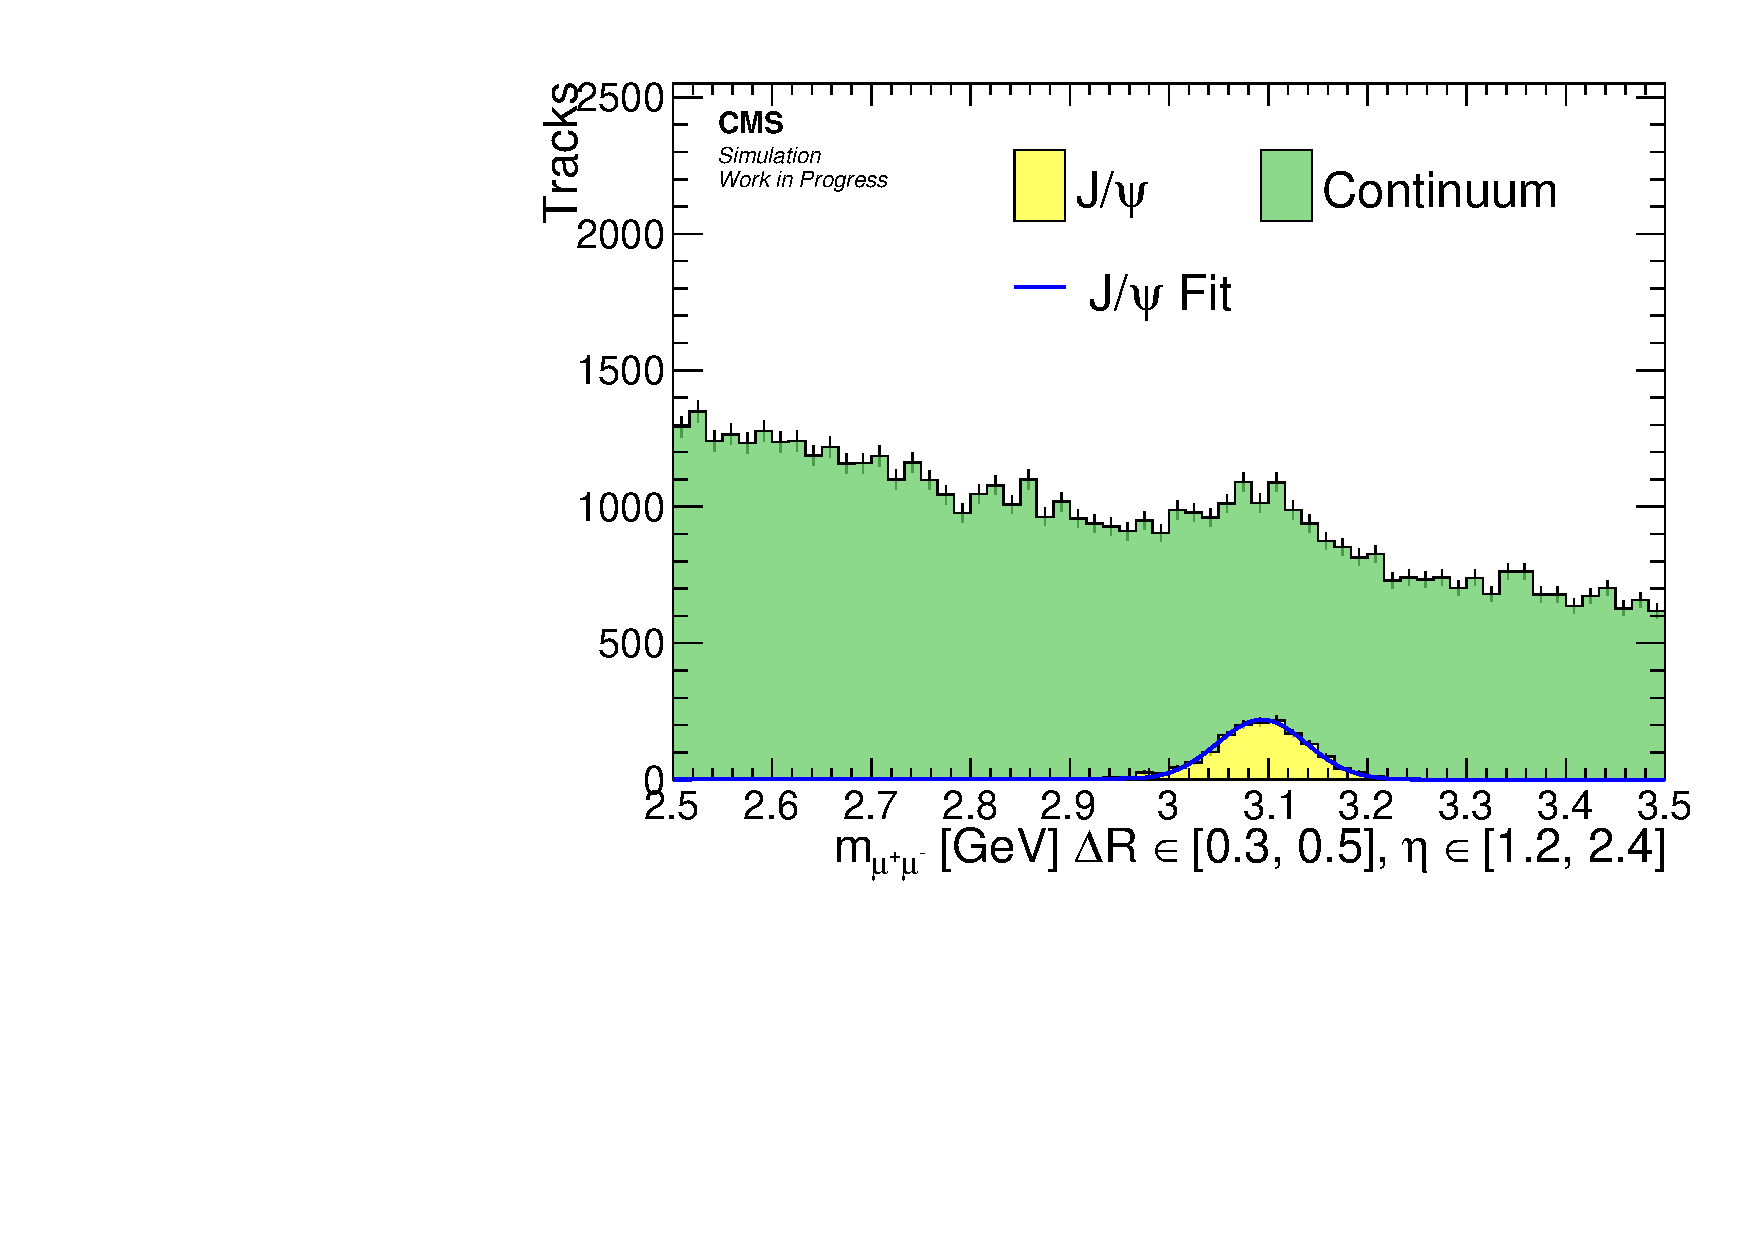
\includegraphics[width=0.32\linewidth]{plots/jpsi_muons_fit_bg_delta_r_single_electron/none_invMass_0.3_0.5_1.2_2.4.pdf} \,
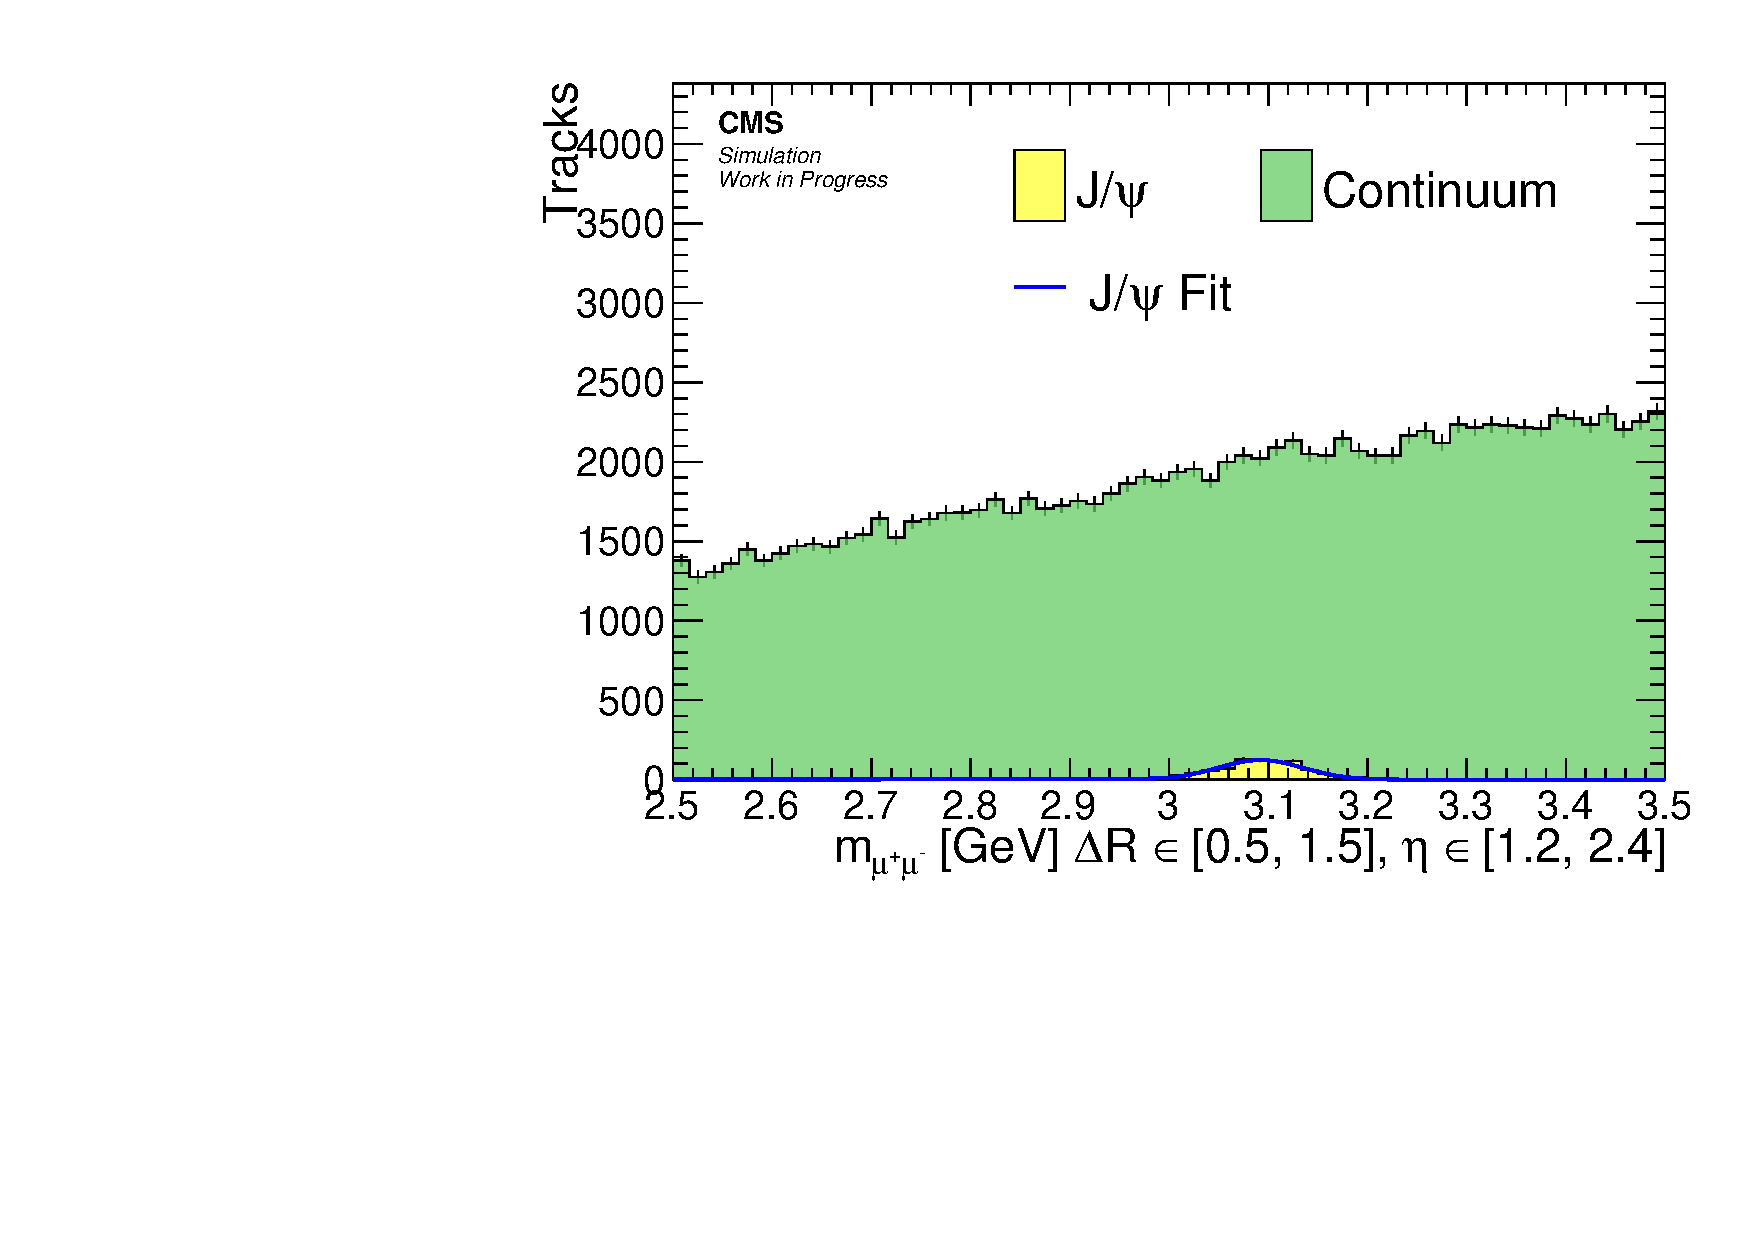
\includegraphics[width=0.32\linewidth]{plots/jpsi_muons_fit_bg_delta_r_single_electron/none_invMass_0.5_1.5_1.2_2.4.pdf} \\
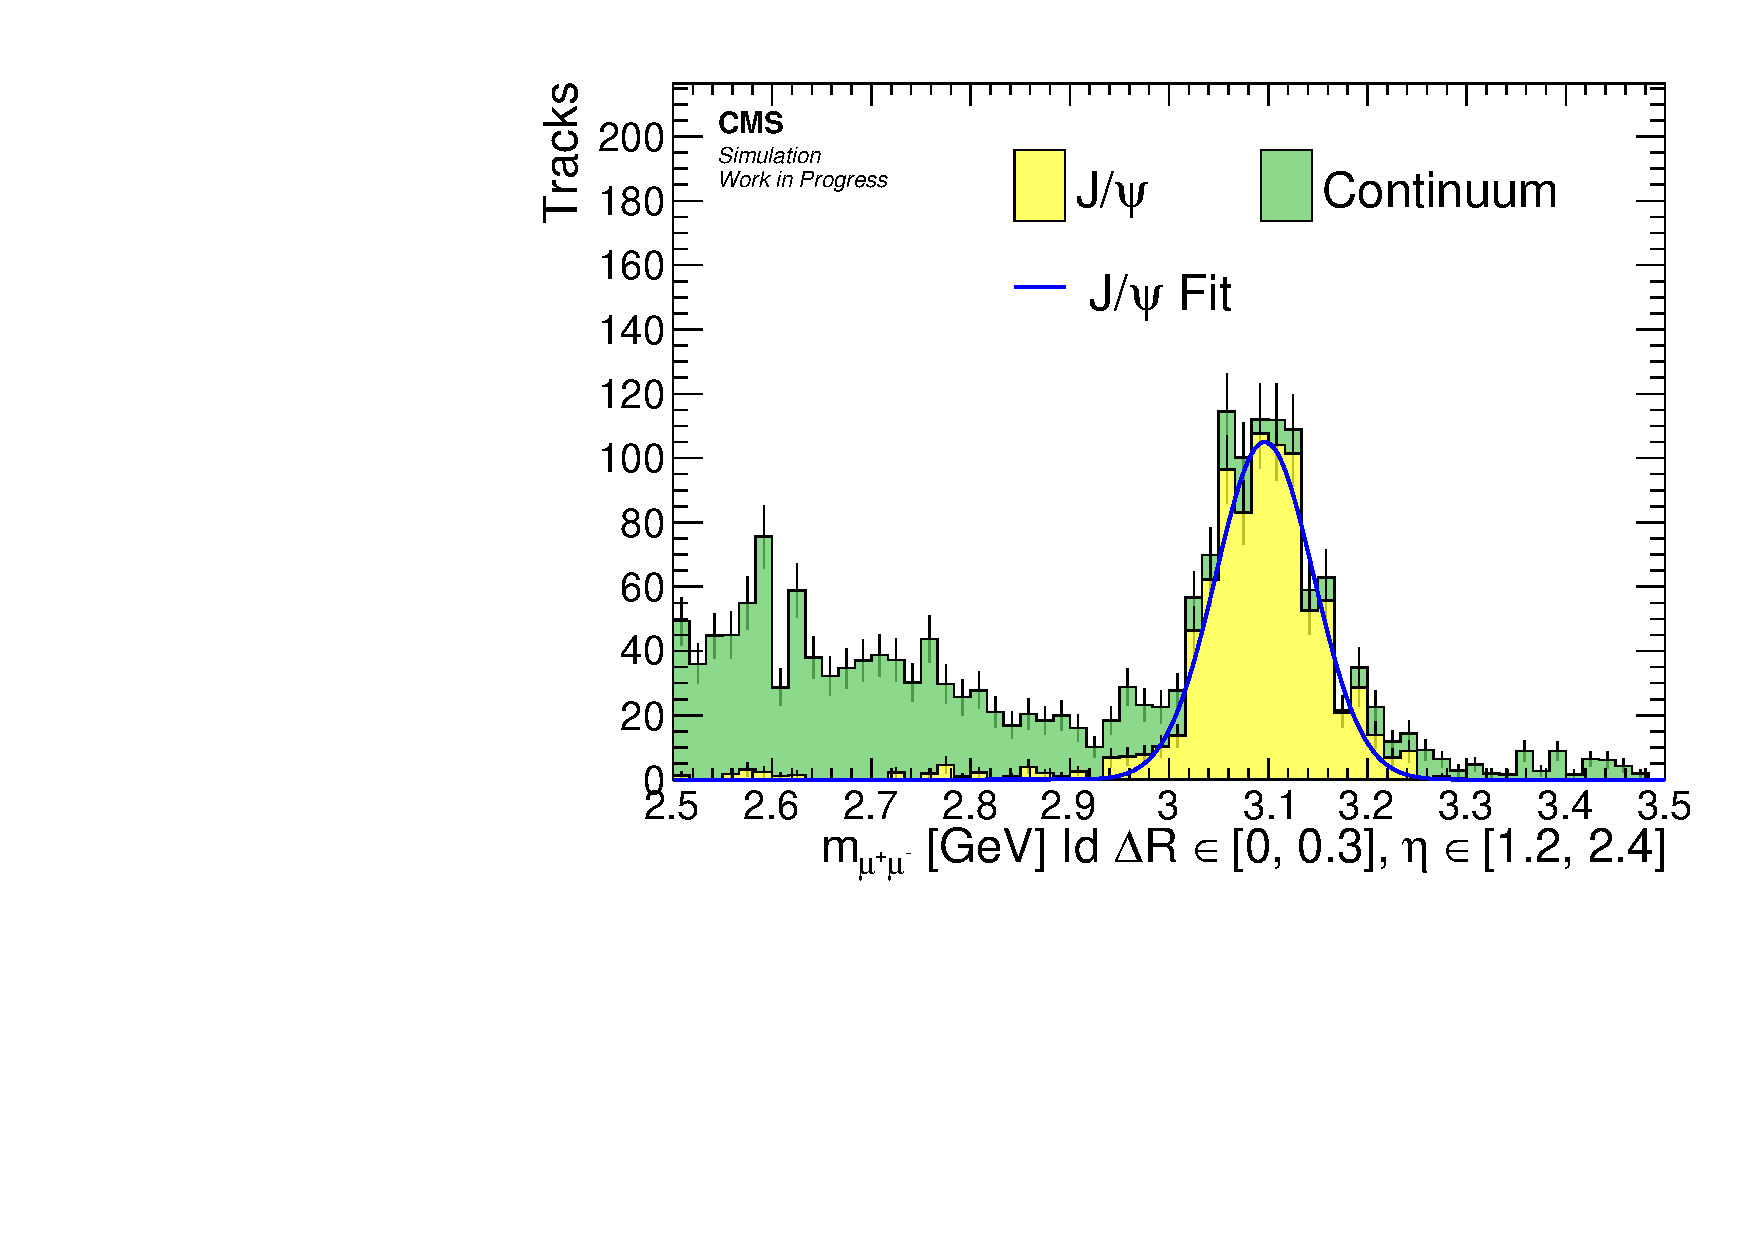
\includegraphics[width=0.32\linewidth]{plots/jpsi_muons_fit_bg_delta_r_single_electron/none_id_invMass_0_0.3_1.2_2.4.pdf} \,
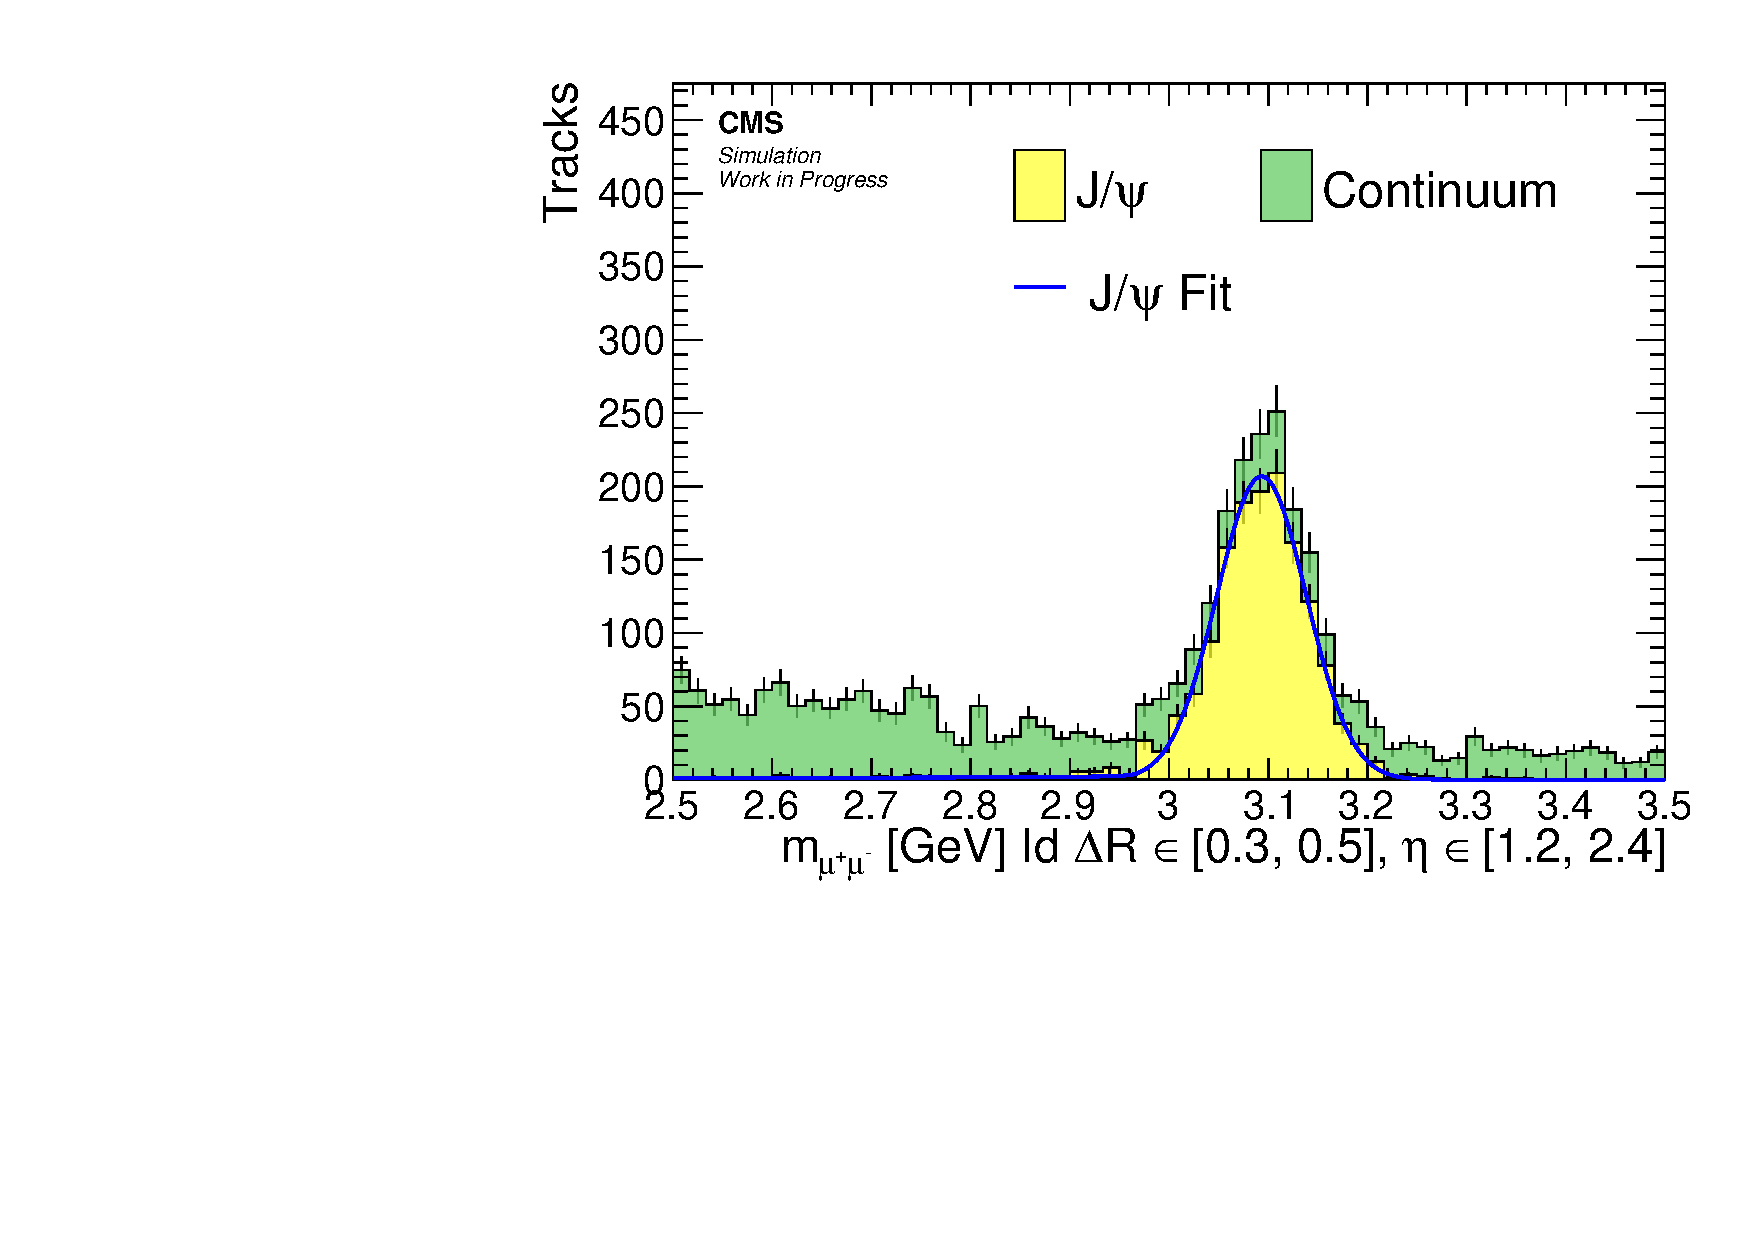
\includegraphics[width=0.32\linewidth]{plots/jpsi_muons_fit_bg_delta_r_single_electron/none_id_invMass_0.3_0.5_1.2_2.4.pdf} \,
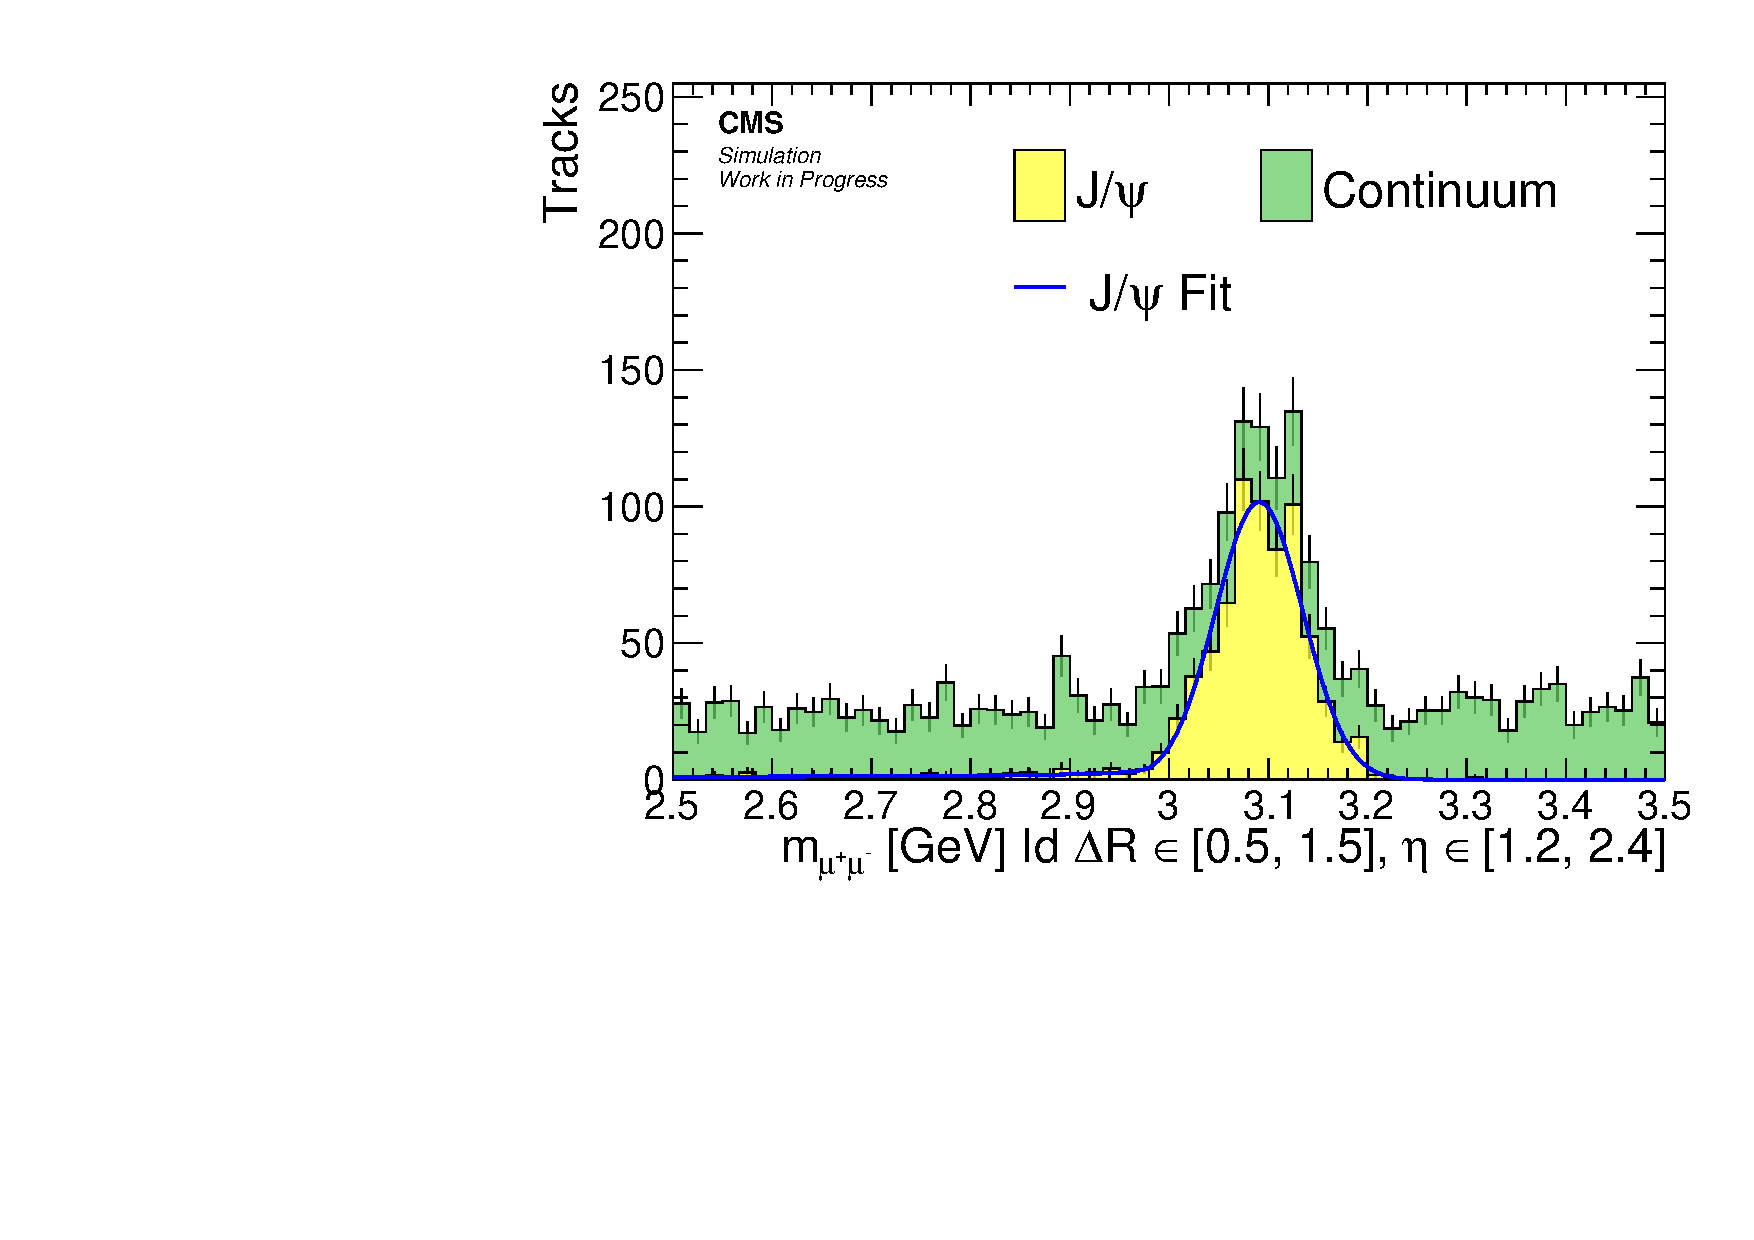
\includegraphics[width=0.32\linewidth]{plots/jpsi_muons_fit_bg_delta_r_single_electron/none_id_invMass_0.5_1.5_1.2_2.4.pdf}  \\
\caption[Simluation endcaps muons fits]{Fits to the tag and probe invariant mass for muons in the endcaps region based on MC. Results are shown for denominator (top) and numerator (bottom) for $0<\DR<0.3$  (left), $0.3<\DR<0.5$ (center), $0.5<\DR<1.5$ (right).}
\label{fig:tb-endcaps-simulation}
\end{figure}

\begin{figure}[!htbp]
\centering
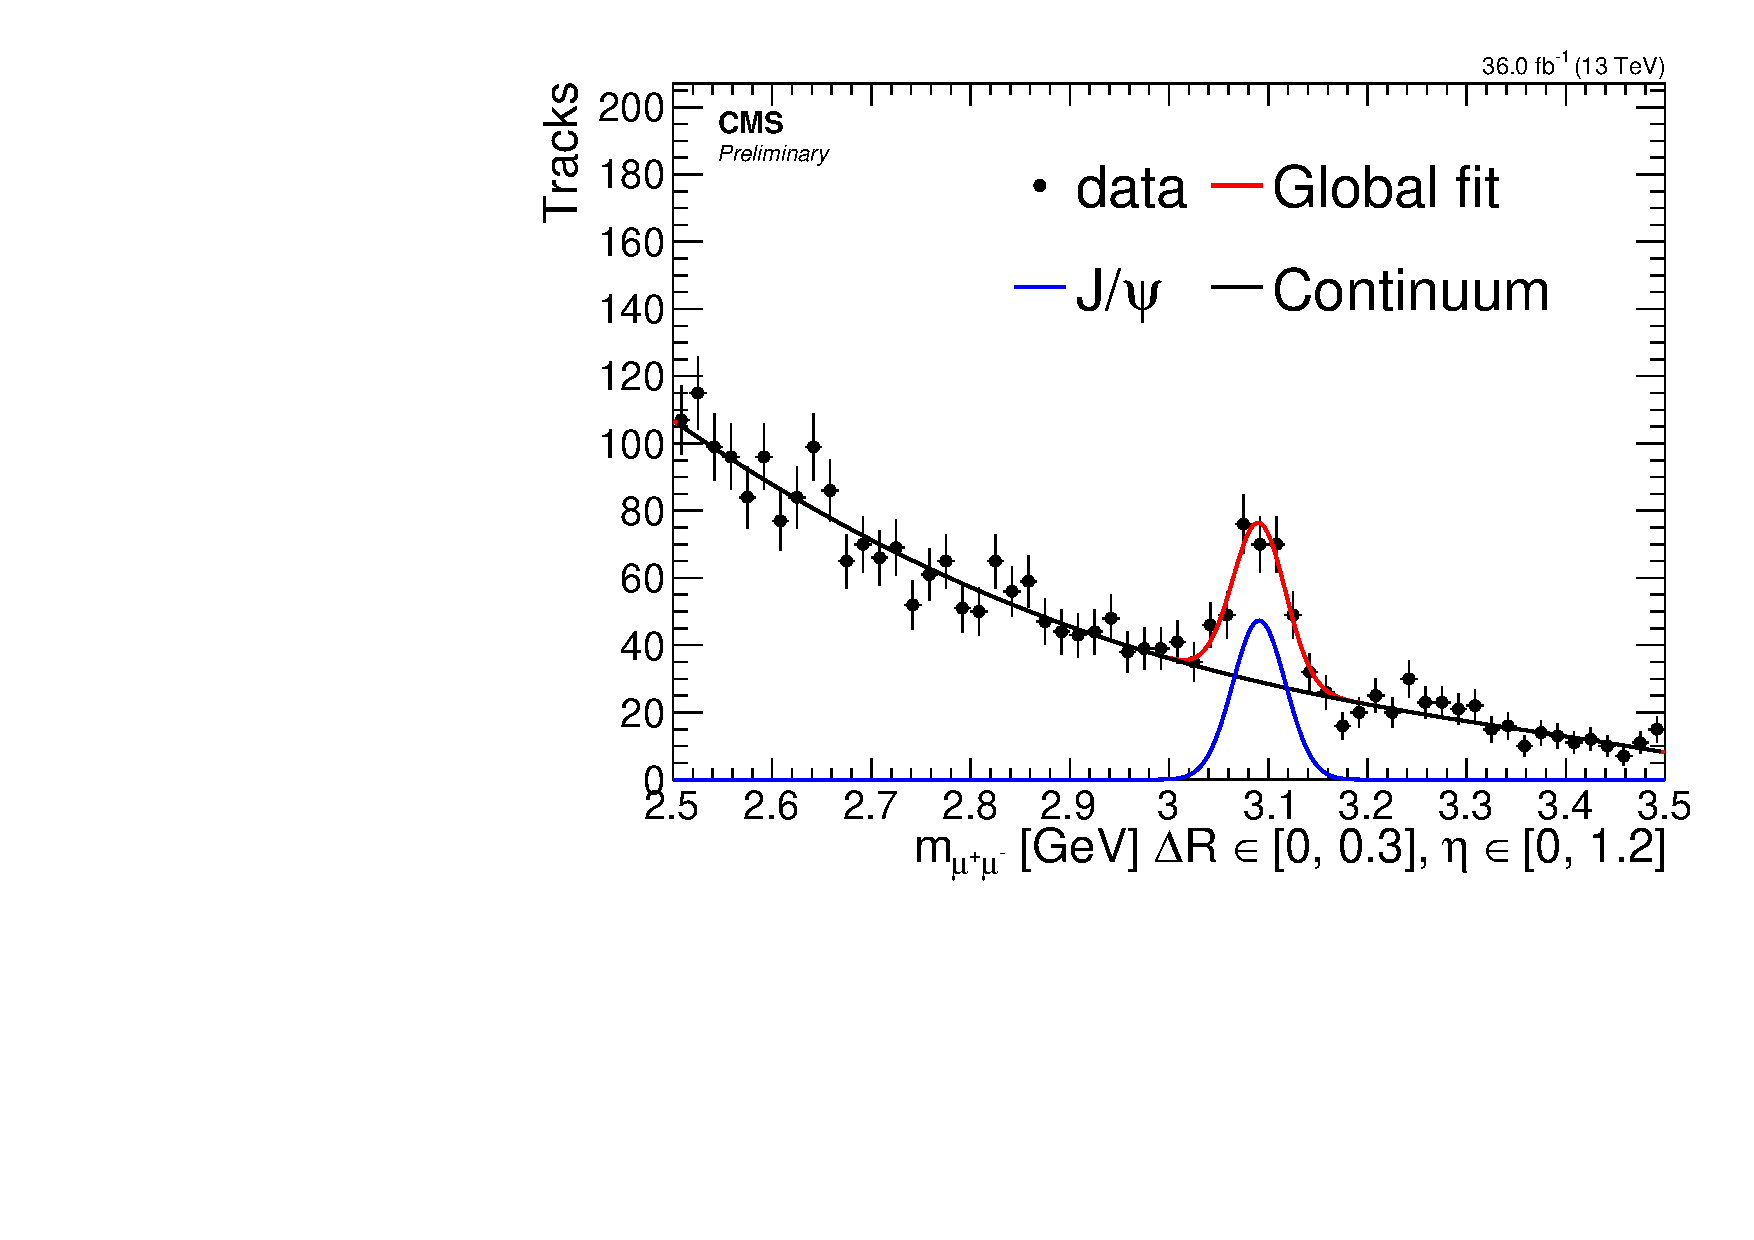
\includegraphics[width=0.32\linewidth]{plots/jpsi_muons_fit_data_delta_r_single_electron/none_invMass_0_0.3_0_1.2.pdf} \,
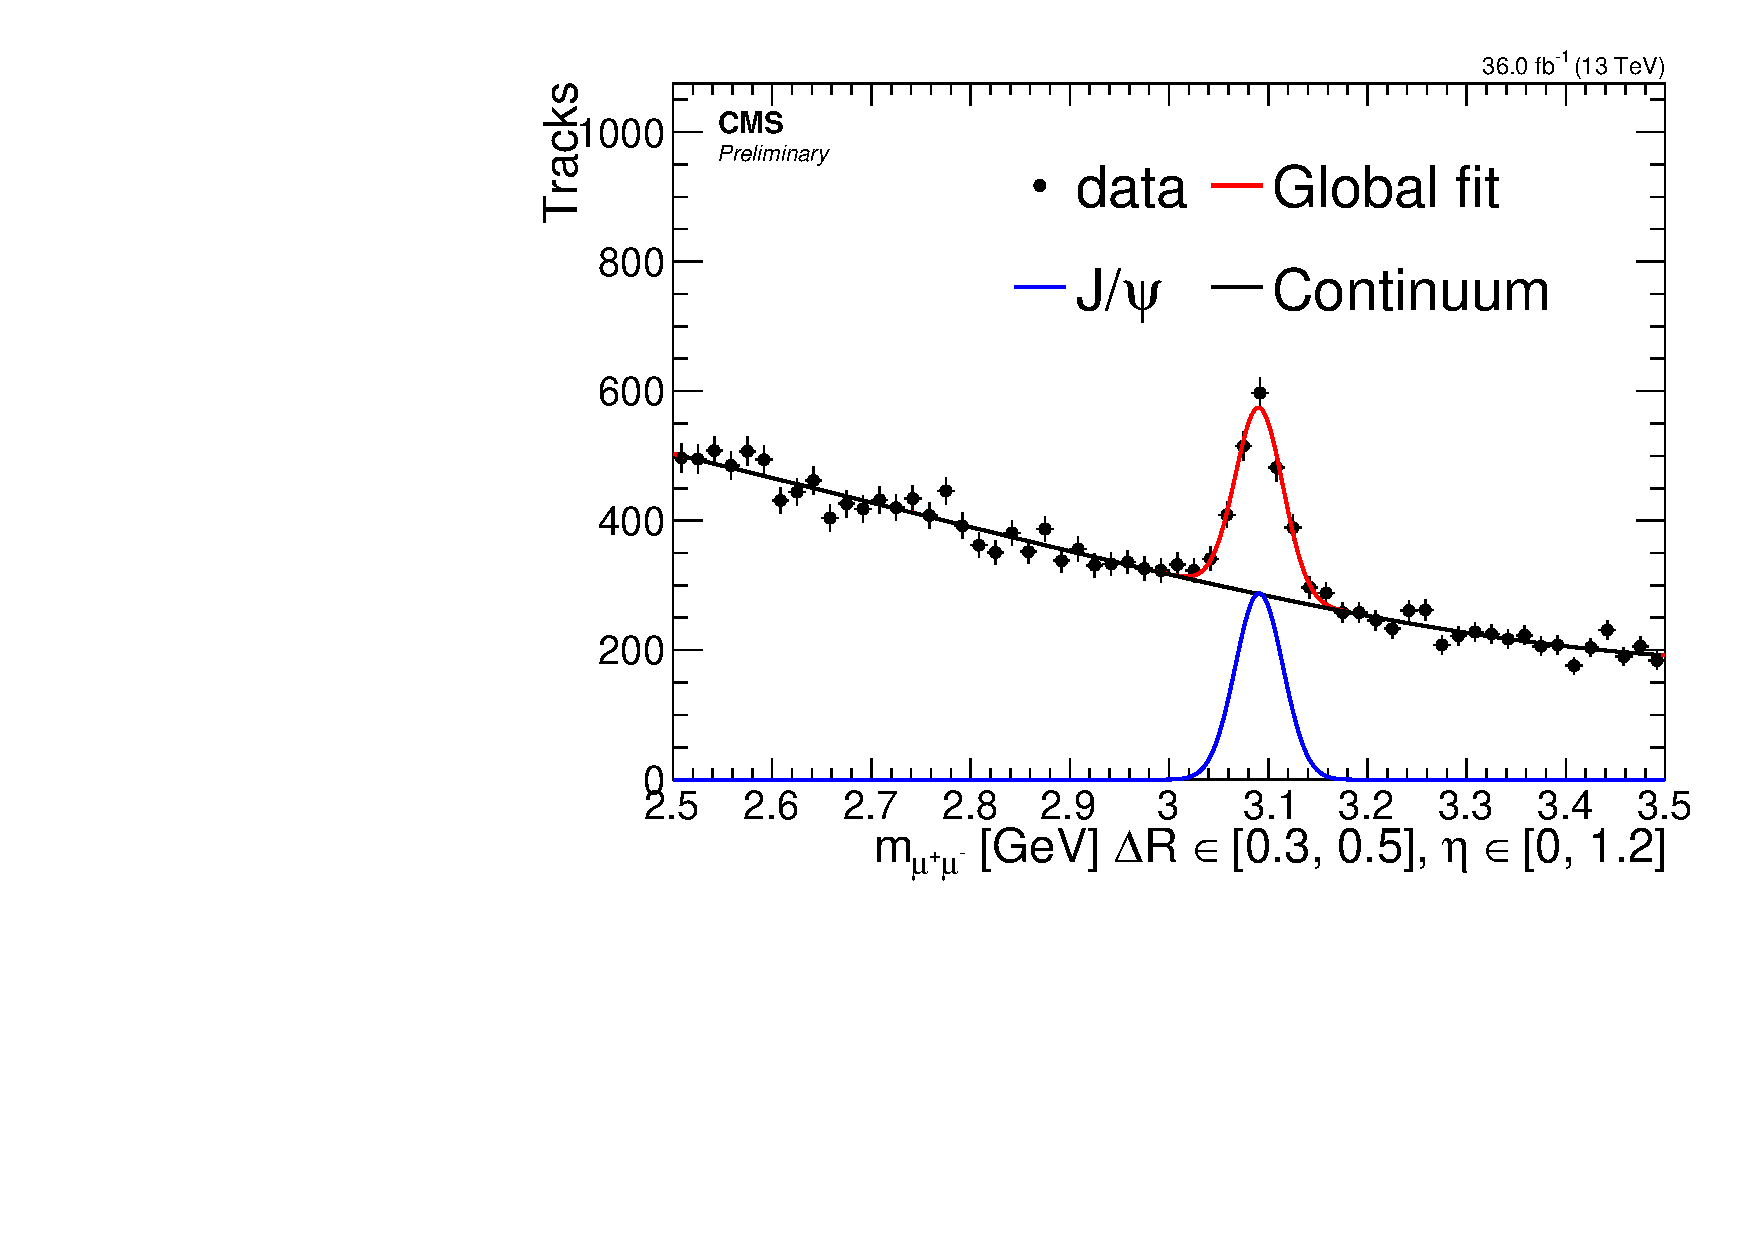
\includegraphics[width=0.32\linewidth]{plots/jpsi_muons_fit_data_delta_r_single_electron/none_invMass_0.3_0.5_0_1.2.pdf}  \,
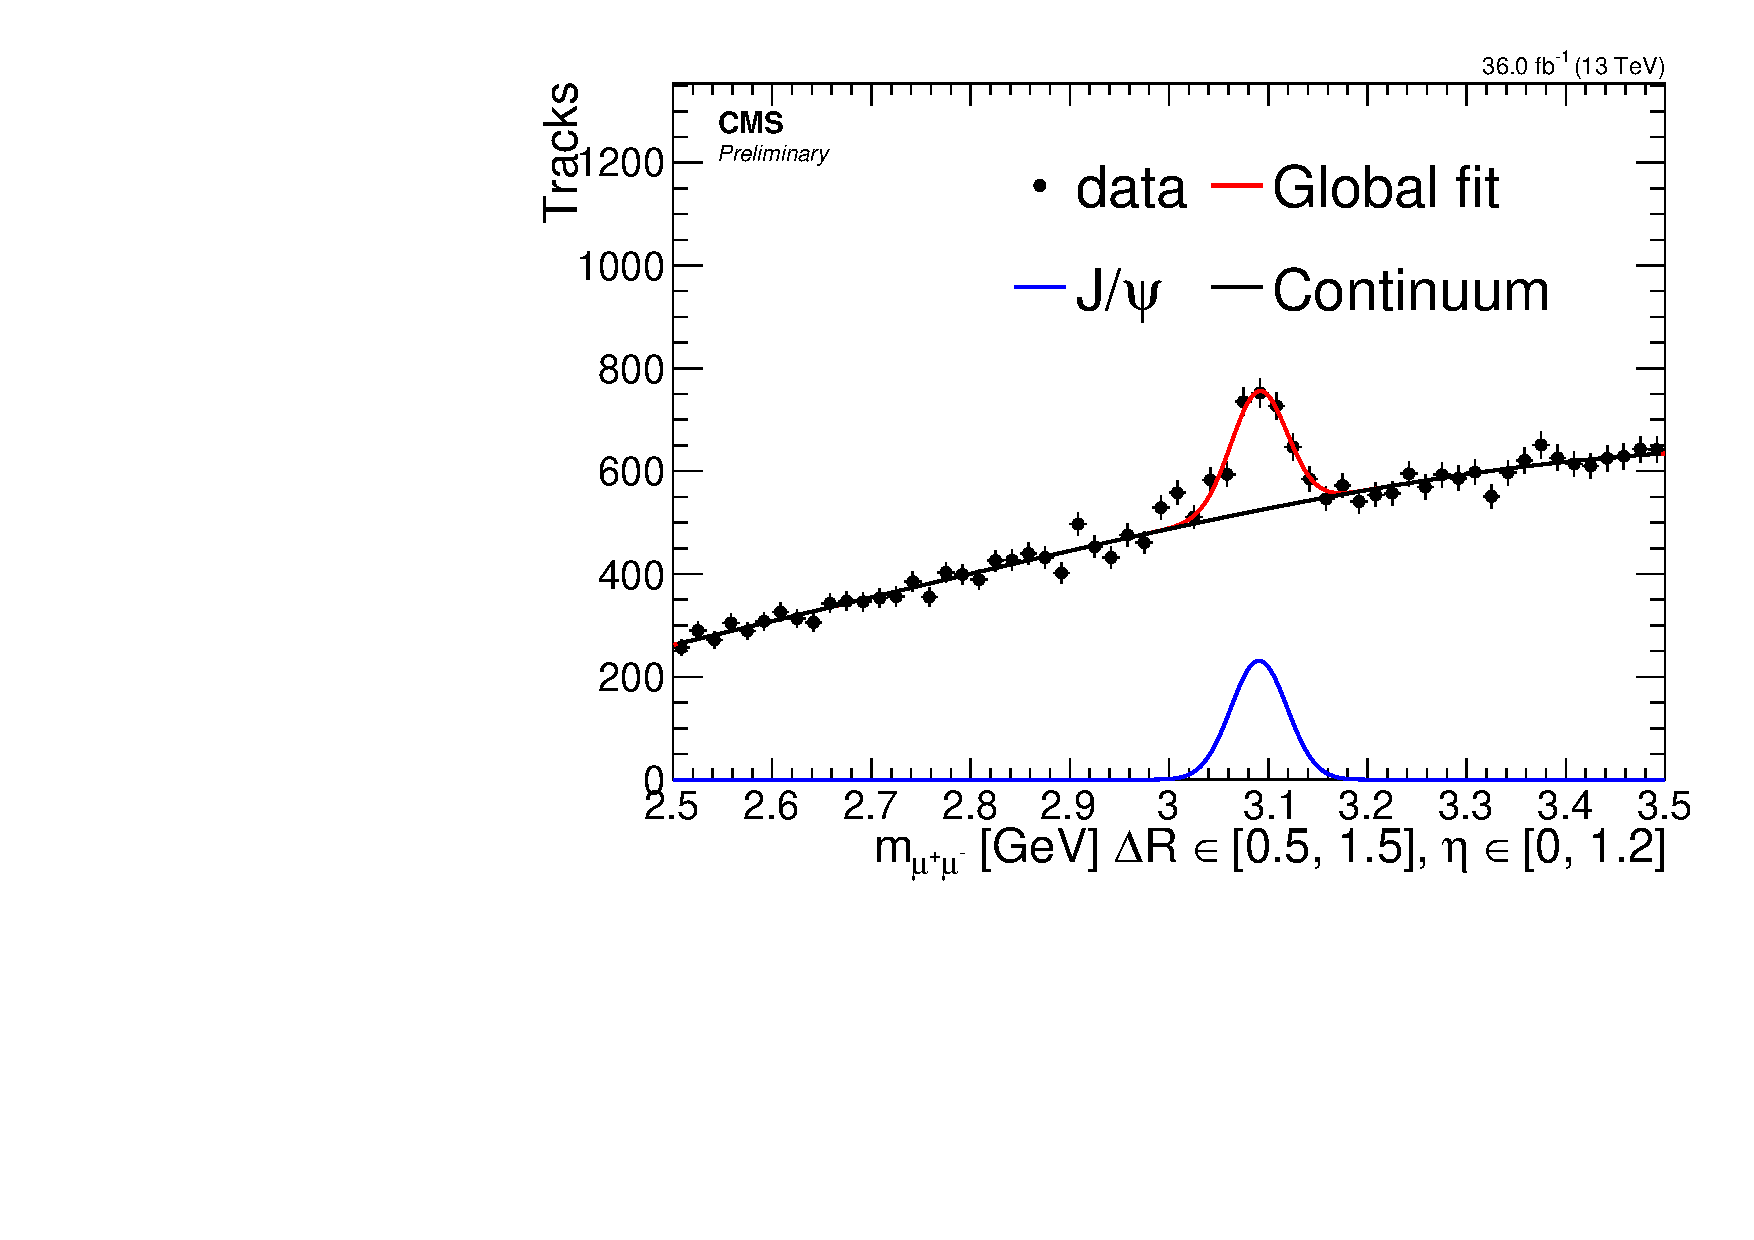
\includegraphics[width=0.32\linewidth]{plots/jpsi_muons_fit_data_delta_r_single_electron/none_invMass_0.5_1.5_0_1.2.pdf} \\
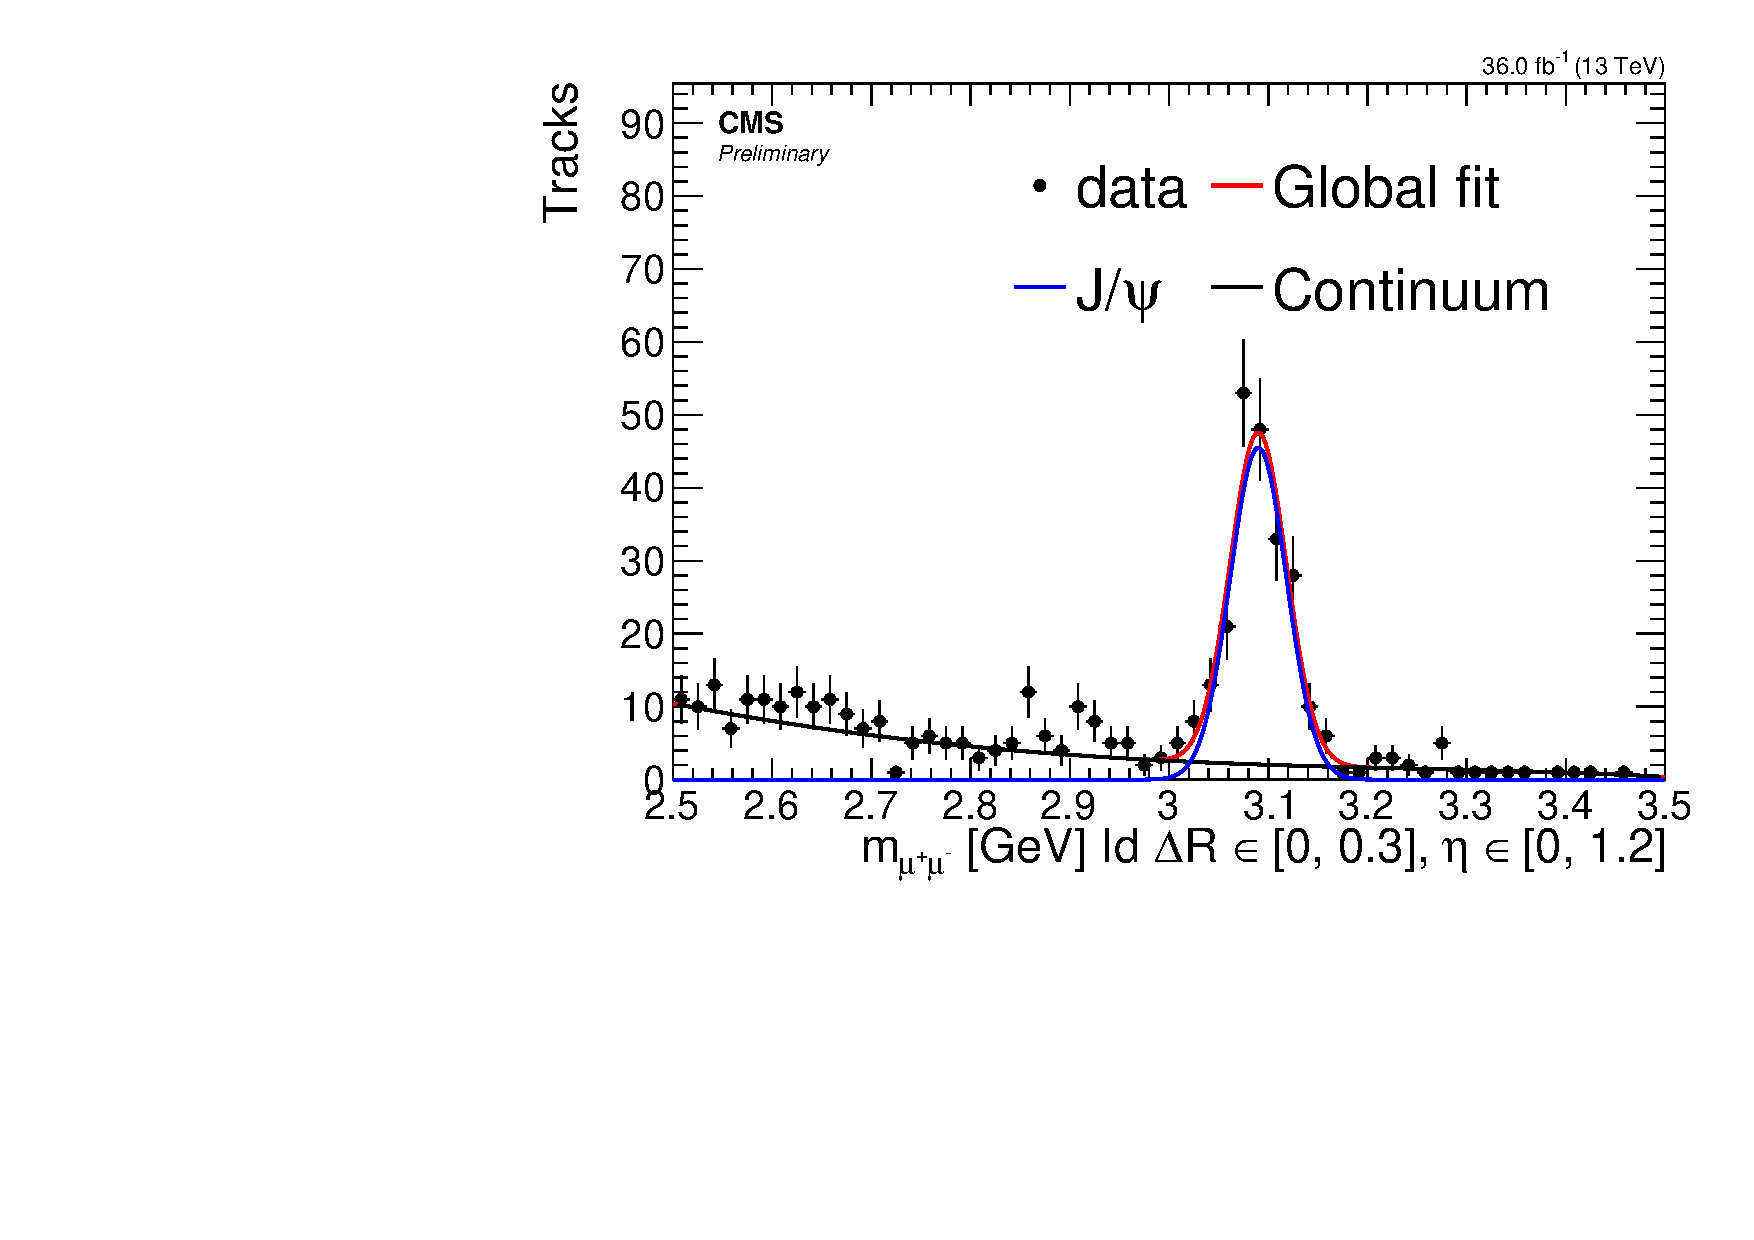
\includegraphics[width=0.32\linewidth]{plots/jpsi_muons_fit_data_delta_r_single_electron/none_id_invMass_0_0.3_0_1.2.pdf} \,
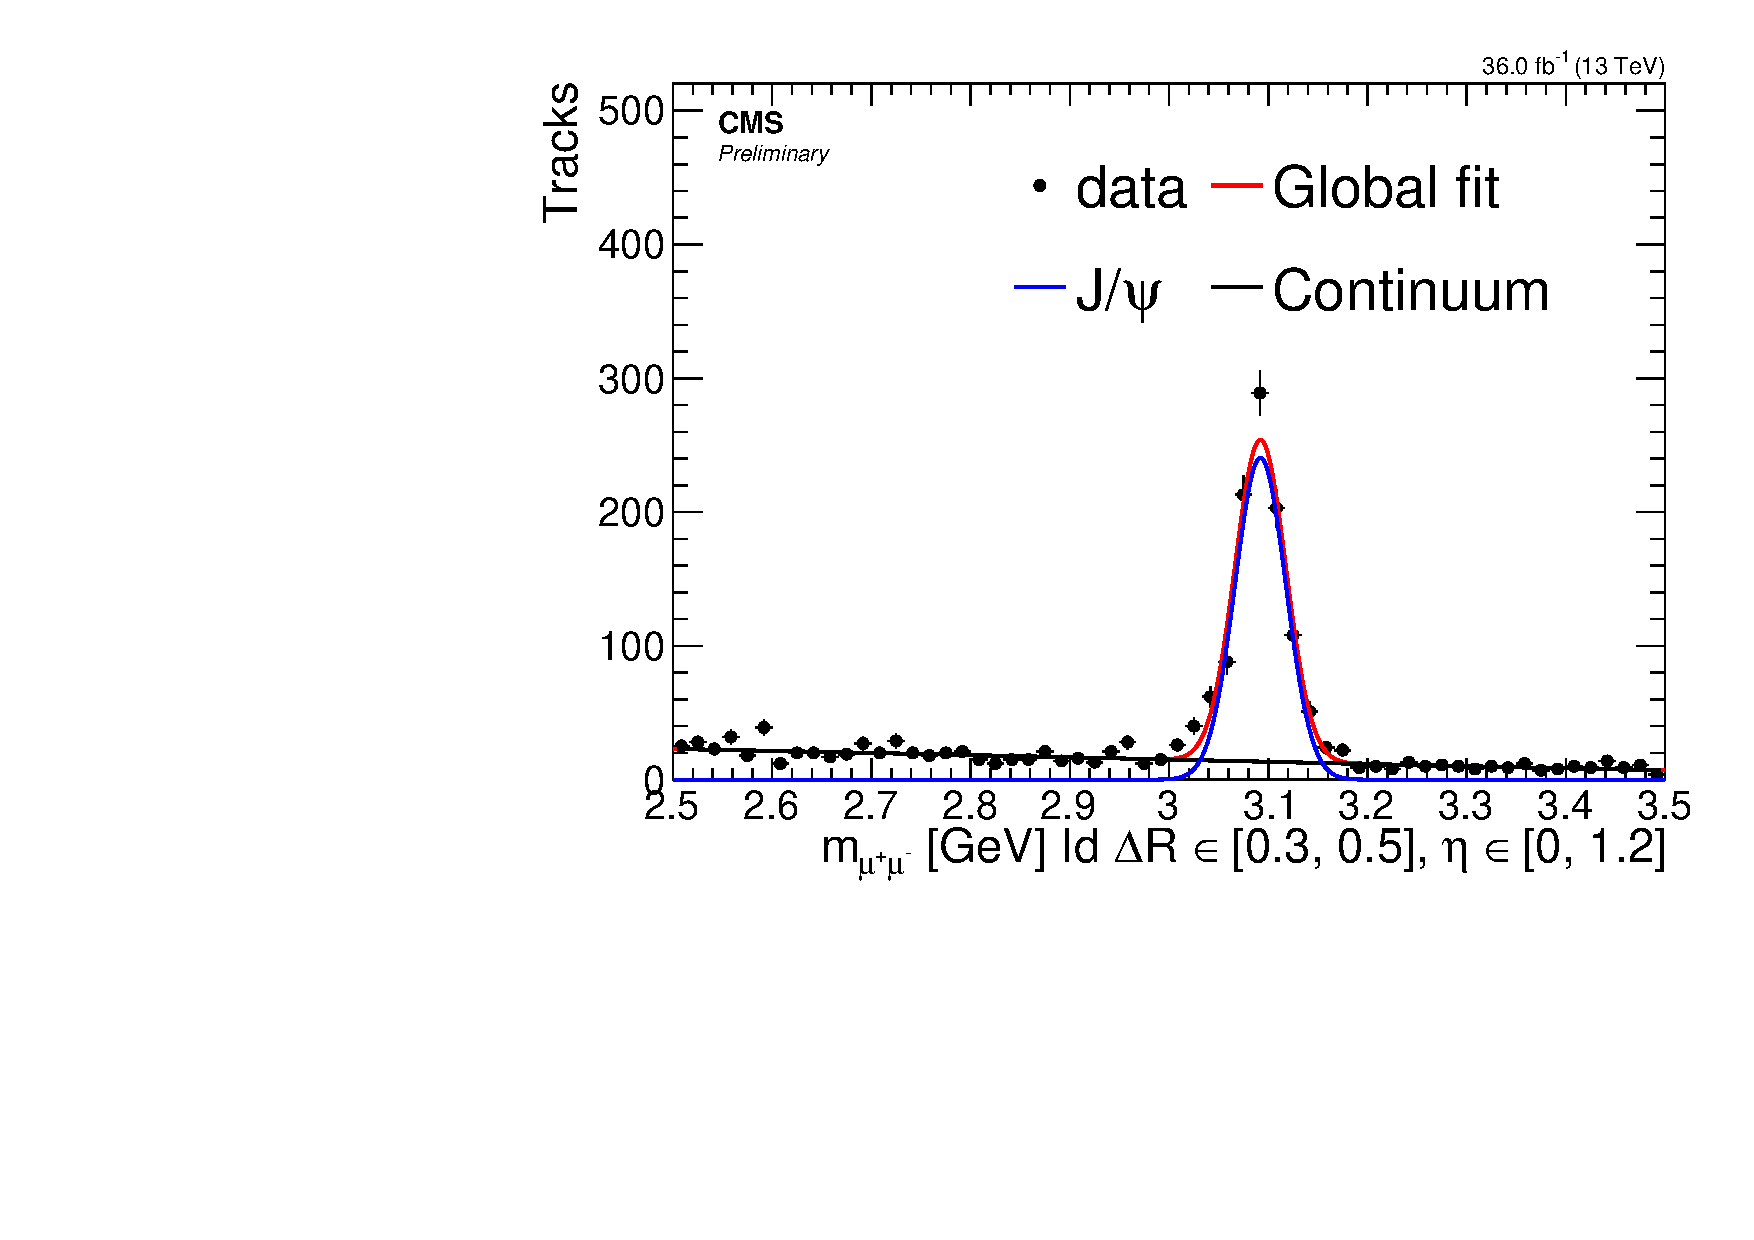
\includegraphics[width=0.32\linewidth]{plots/jpsi_muons_fit_data_delta_r_single_electron/none_id_invMass_0.3_0.5_0_1.2.pdf}  \,
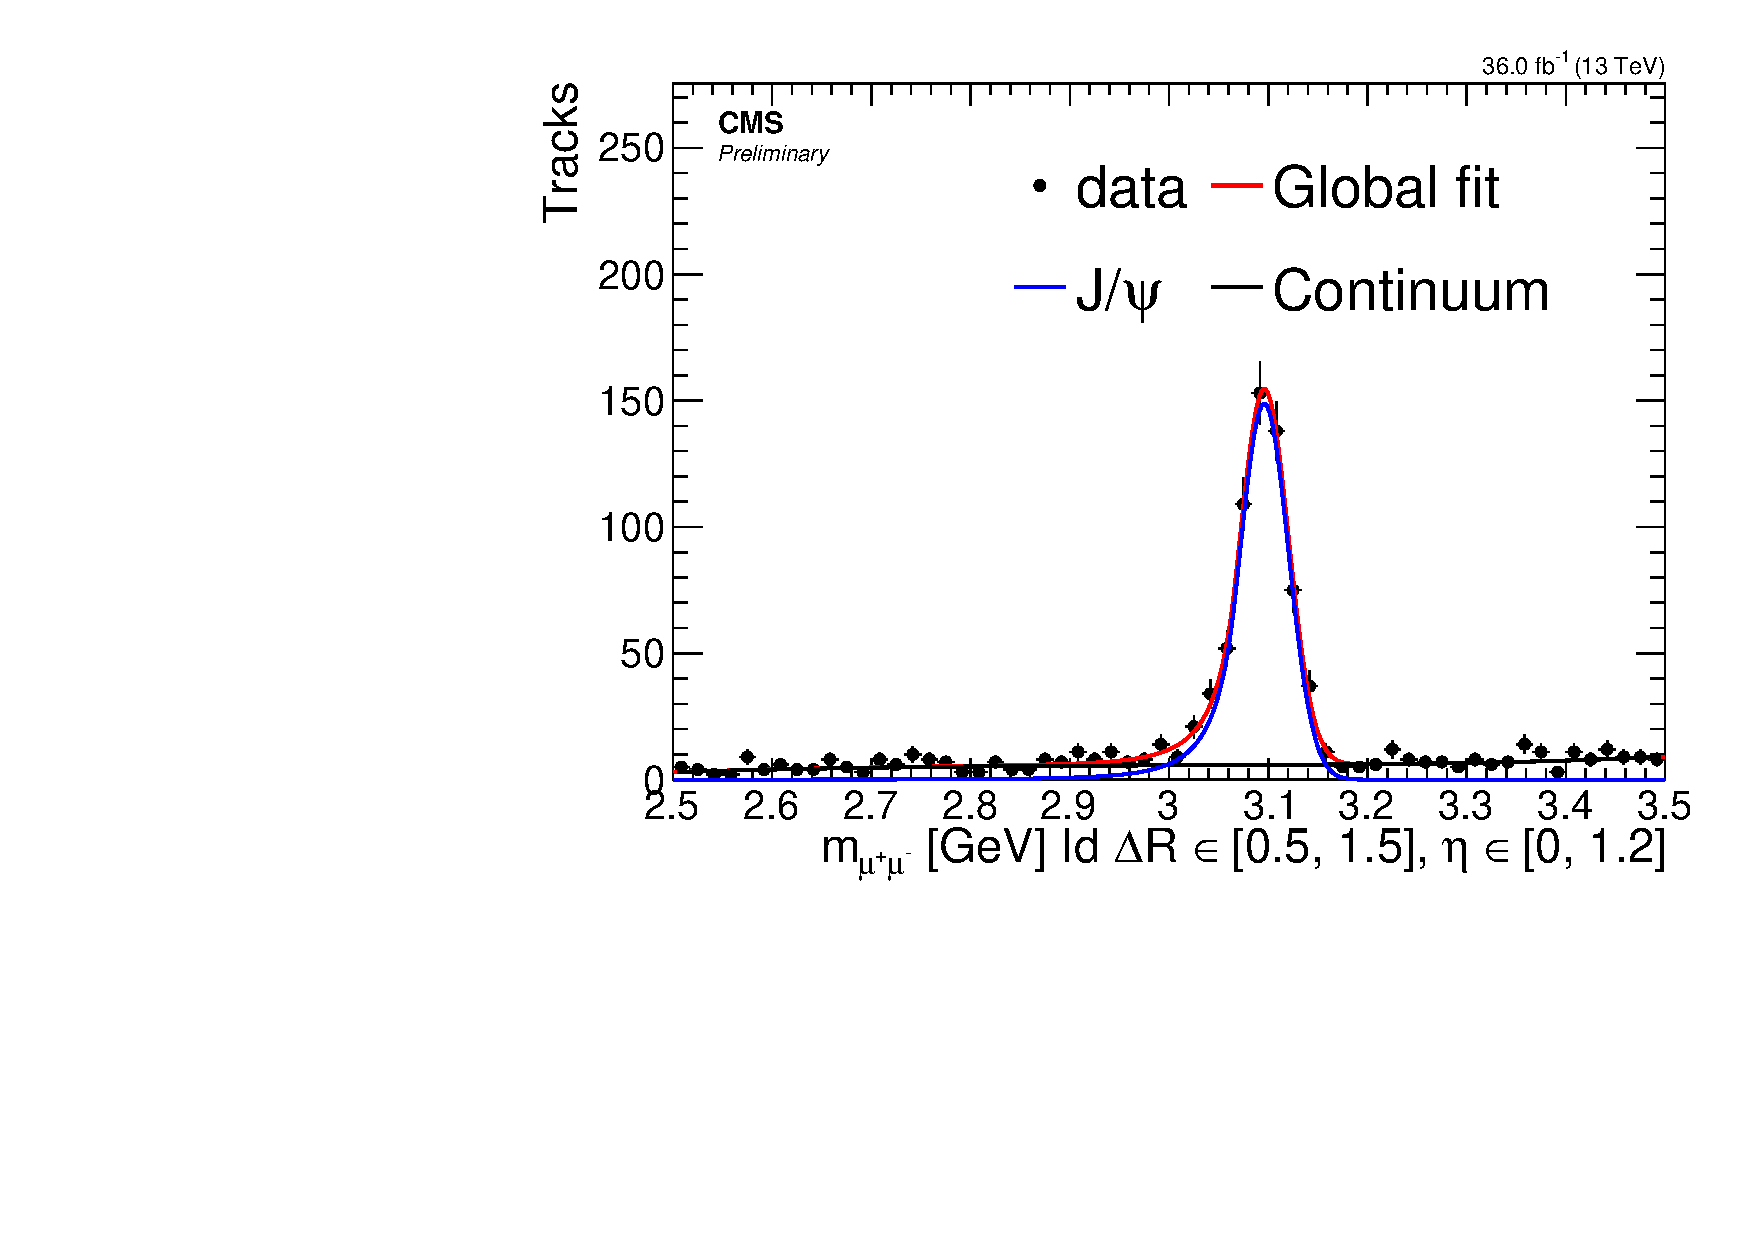
\includegraphics[width=0.32\linewidth]{plots/jpsi_muons_fit_data_delta_r_single_electron/none_id_invMass_0.5_1.5_0_1.2.pdf} \\
\caption[Data barrel muons fits]{Fits to the tag and probe invariant mass for muons in the barrel region based on data. Results are shown for denominator (top) and numerator (bottom) for $0<\DR<0.3$  (left), $0.3<\DR<0.5$ (center), $0.5<\DR<1.5$ (right).}
\label{fig:tb-barrel-data}
\end{figure}

\begin{figure}[!htbp]
\centering
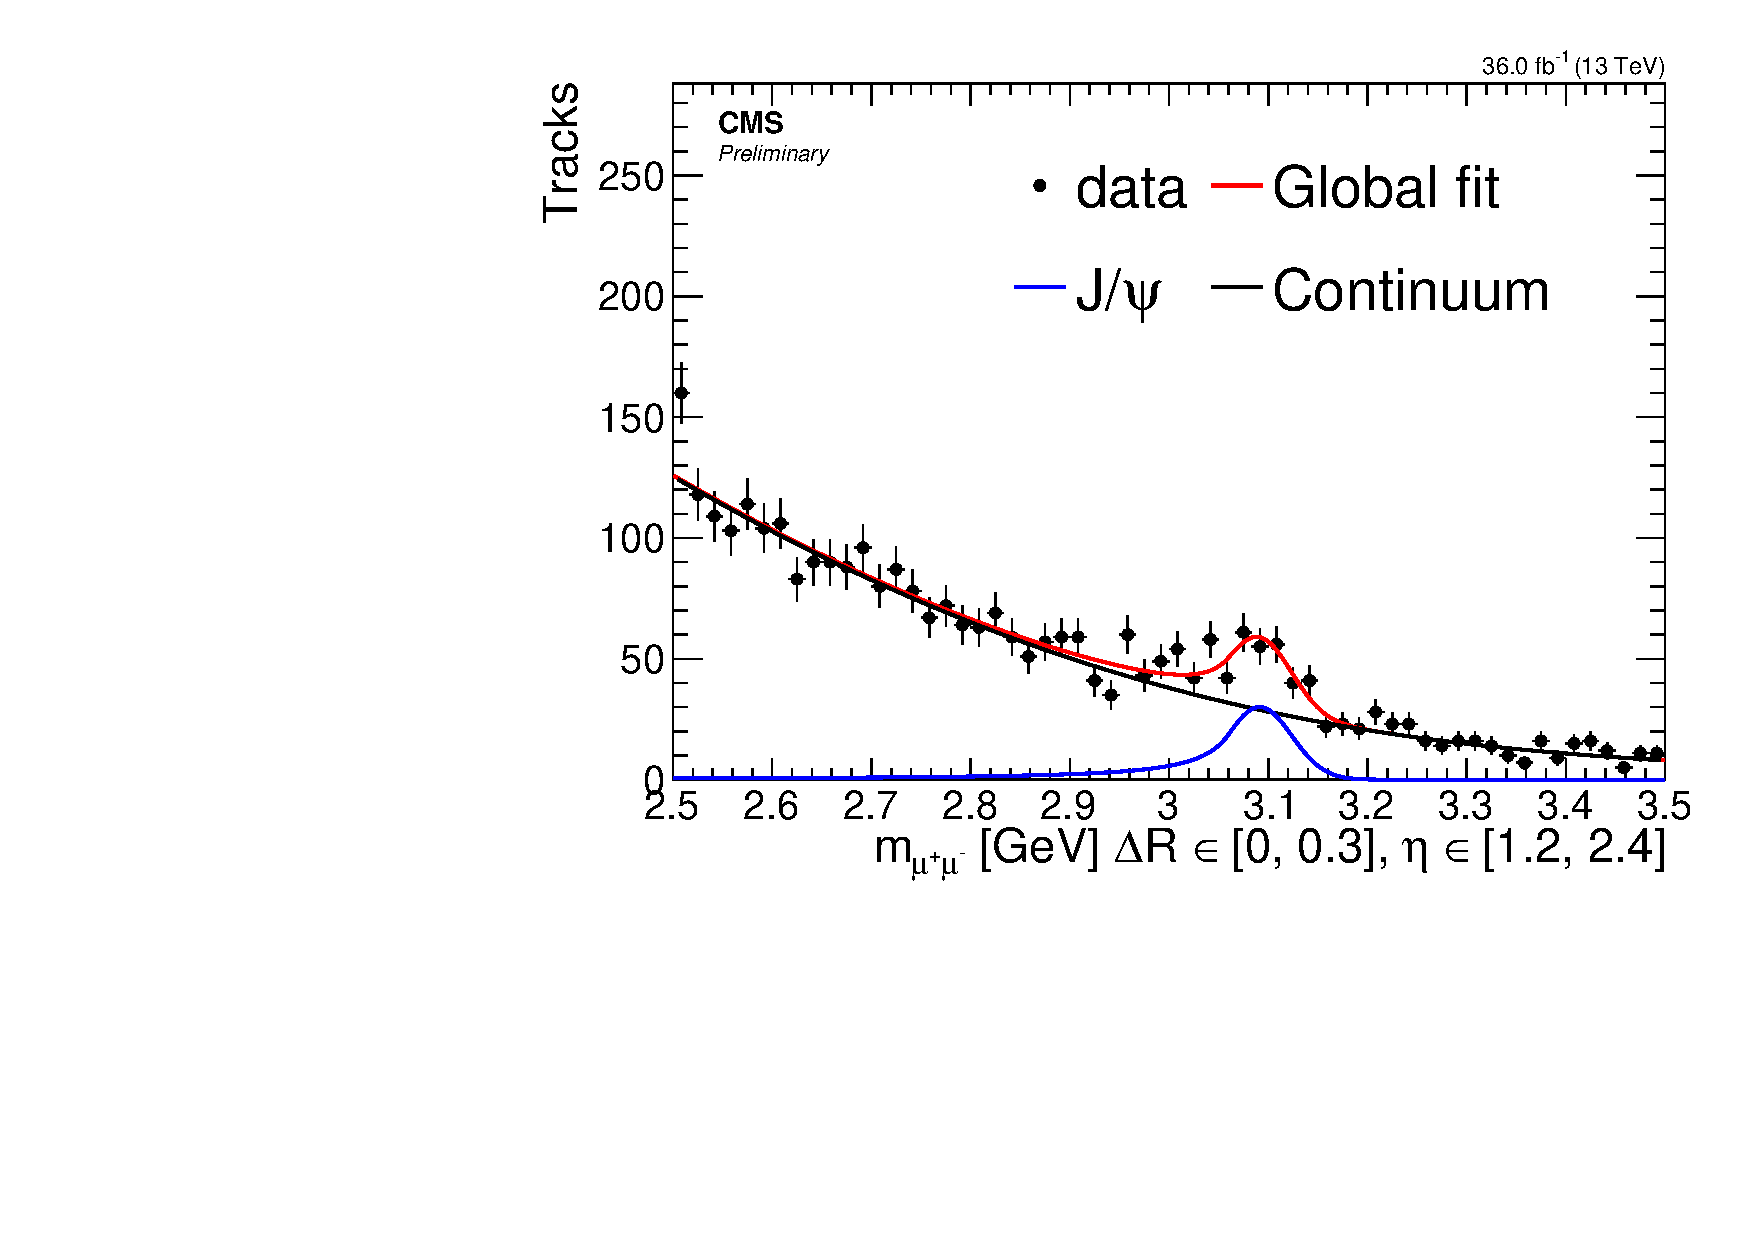
\includegraphics[width=0.32\linewidth]{plots/jpsi_muons_fit_data_delta_r_single_electron/none_invMass_0_0.3_1.2_2.4.pdf} \,
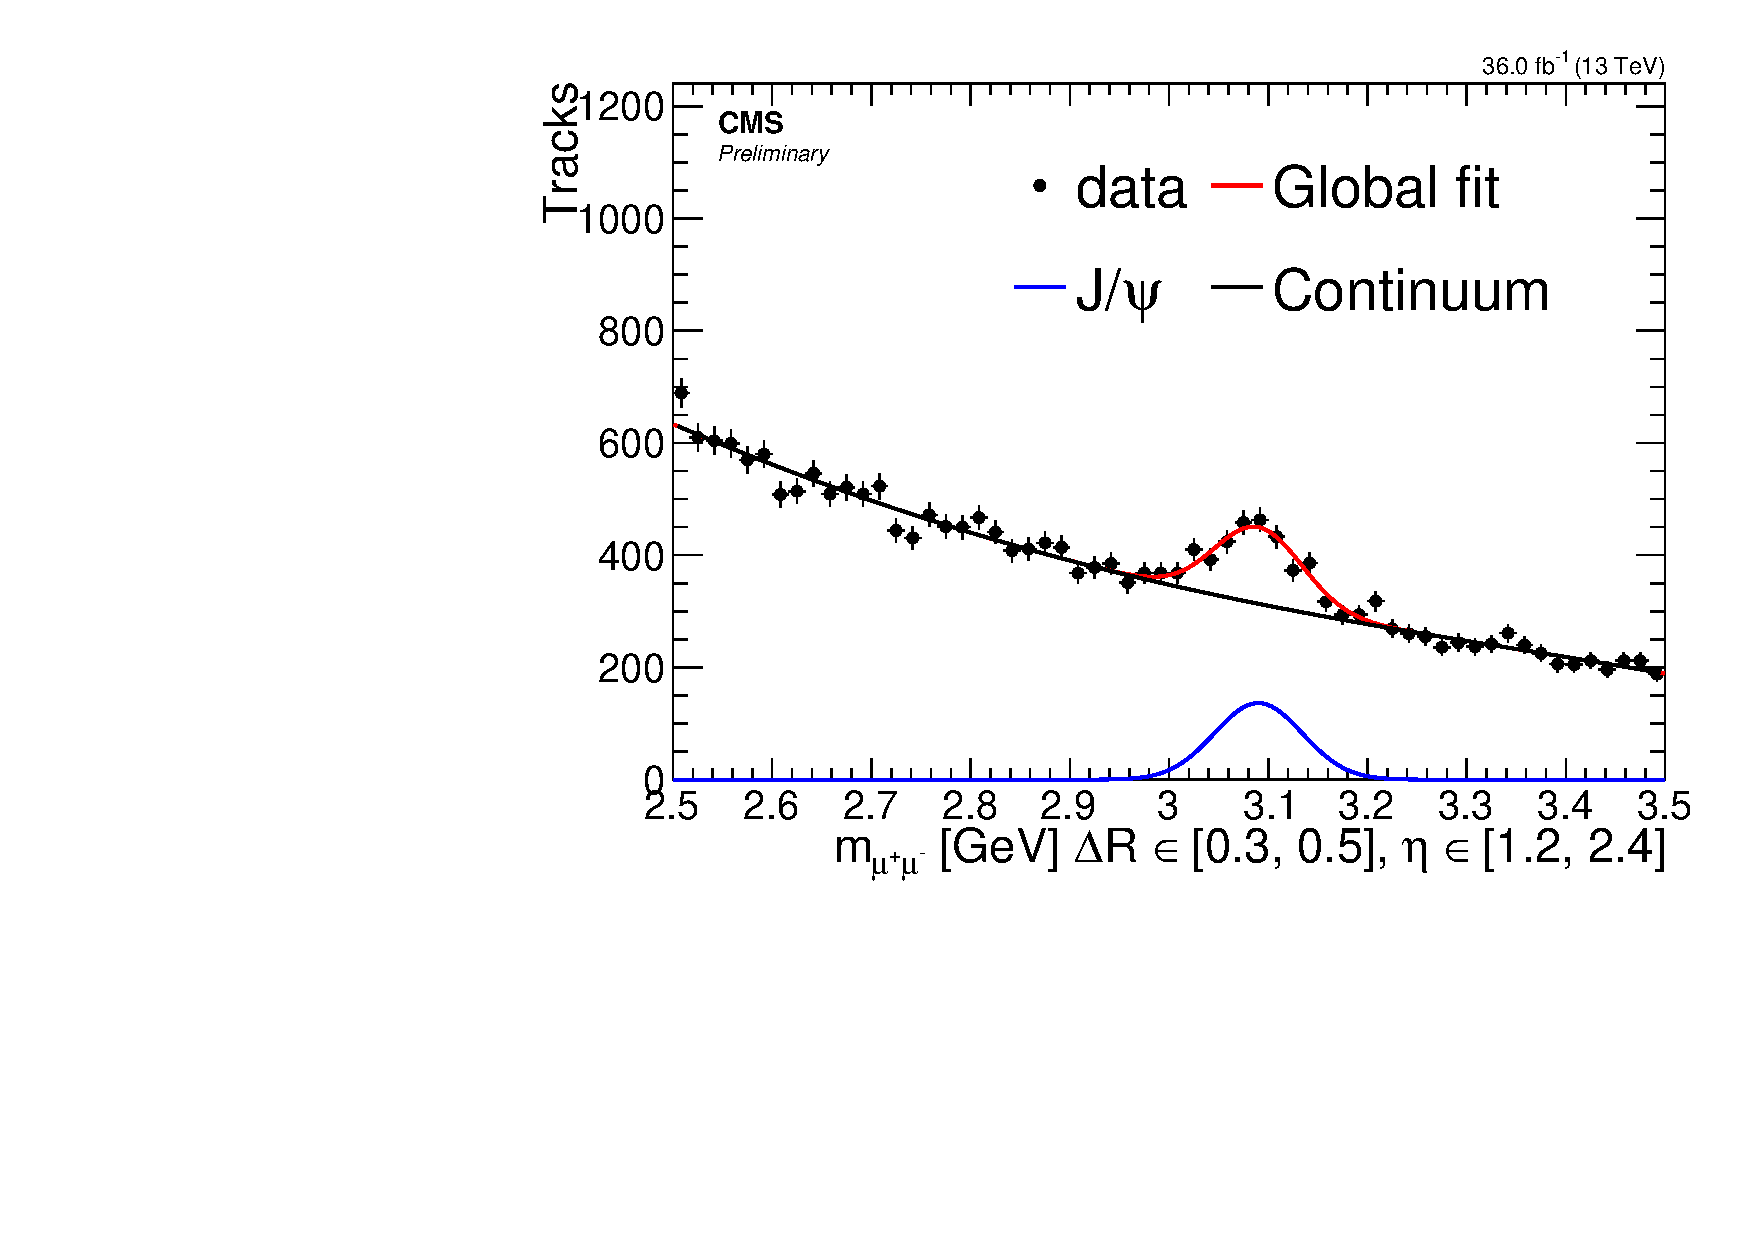
\includegraphics[width=0.32\linewidth]{plots/jpsi_muons_fit_data_delta_r_single_electron/none_invMass_0.3_0.5_1.2_2.4.pdf} \,
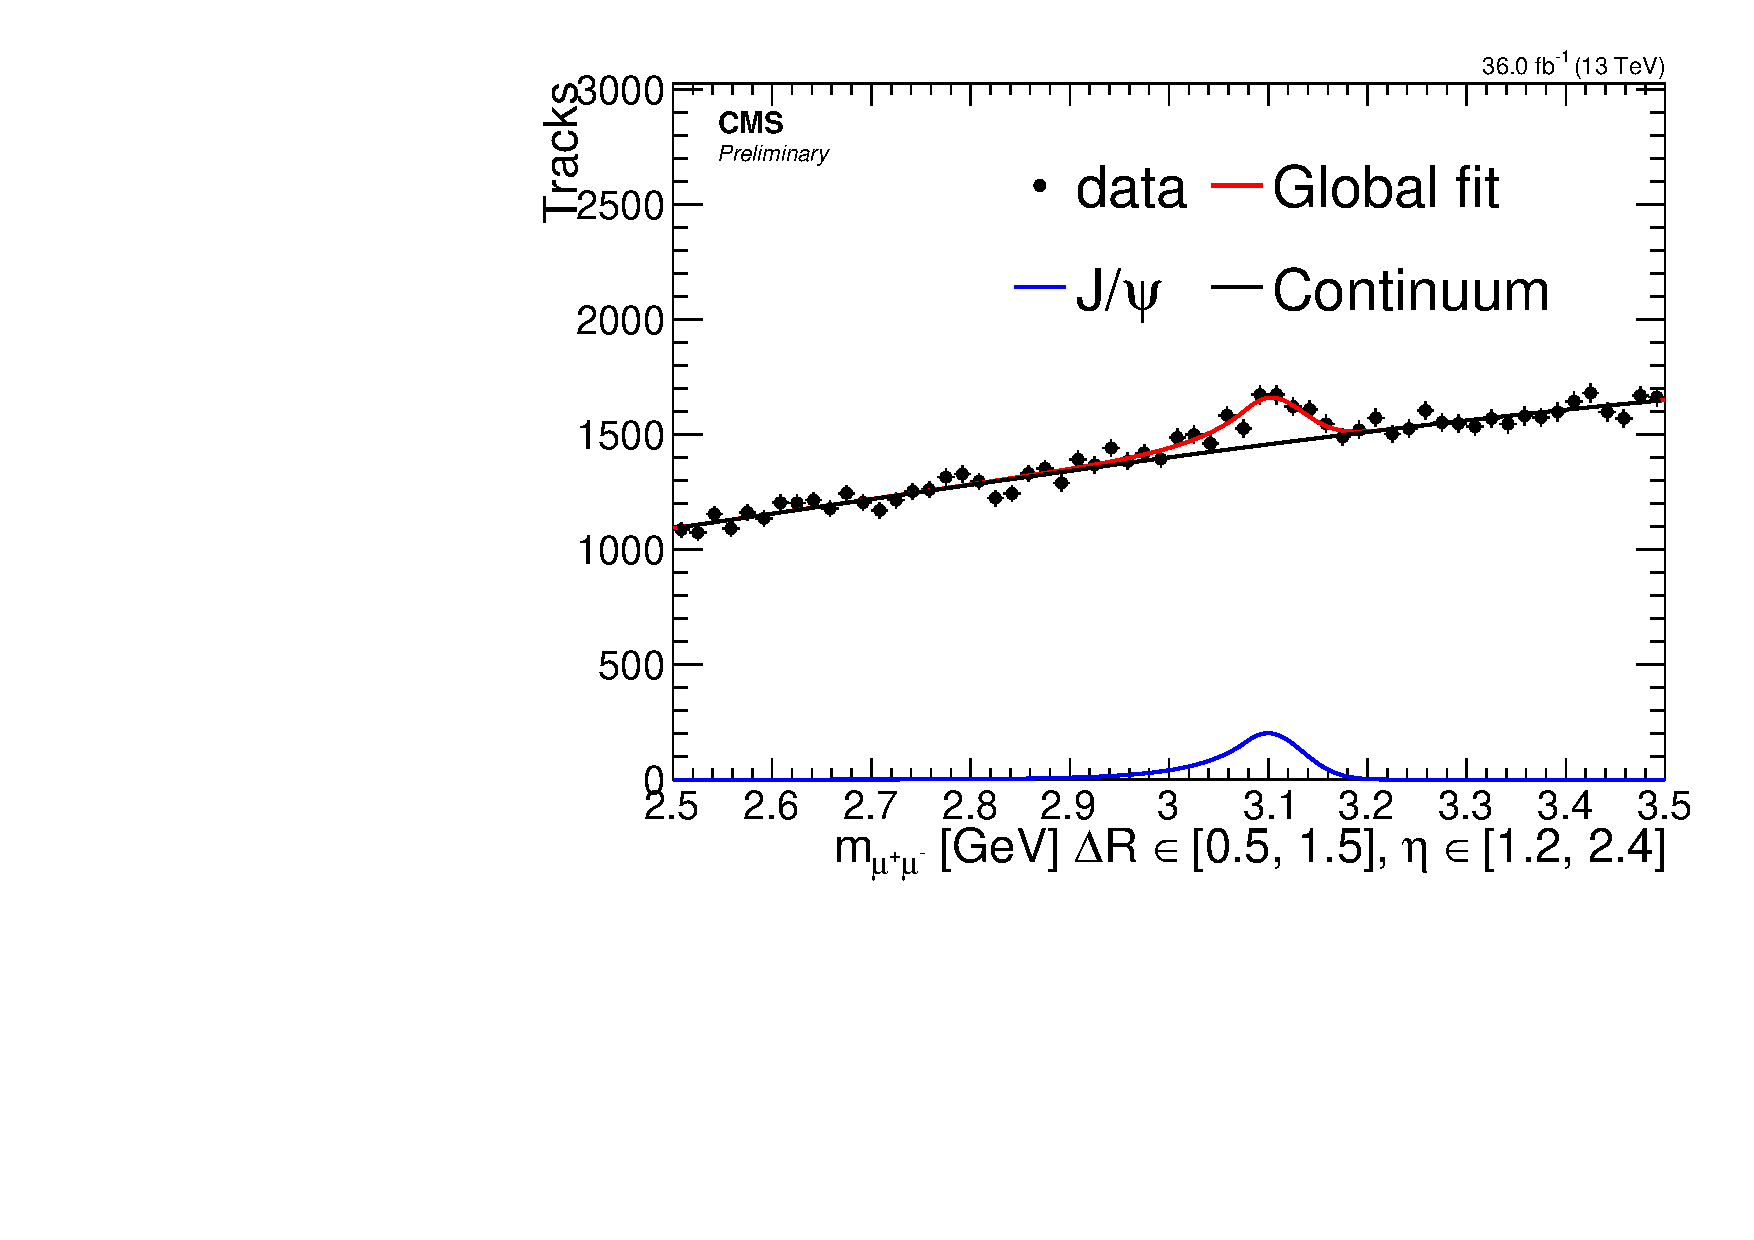
\includegraphics[width=0.32\linewidth]{plots/jpsi_muons_fit_data_delta_r_single_electron/none_invMass_0.5_1.5_1.2_2.4.pdf} \\
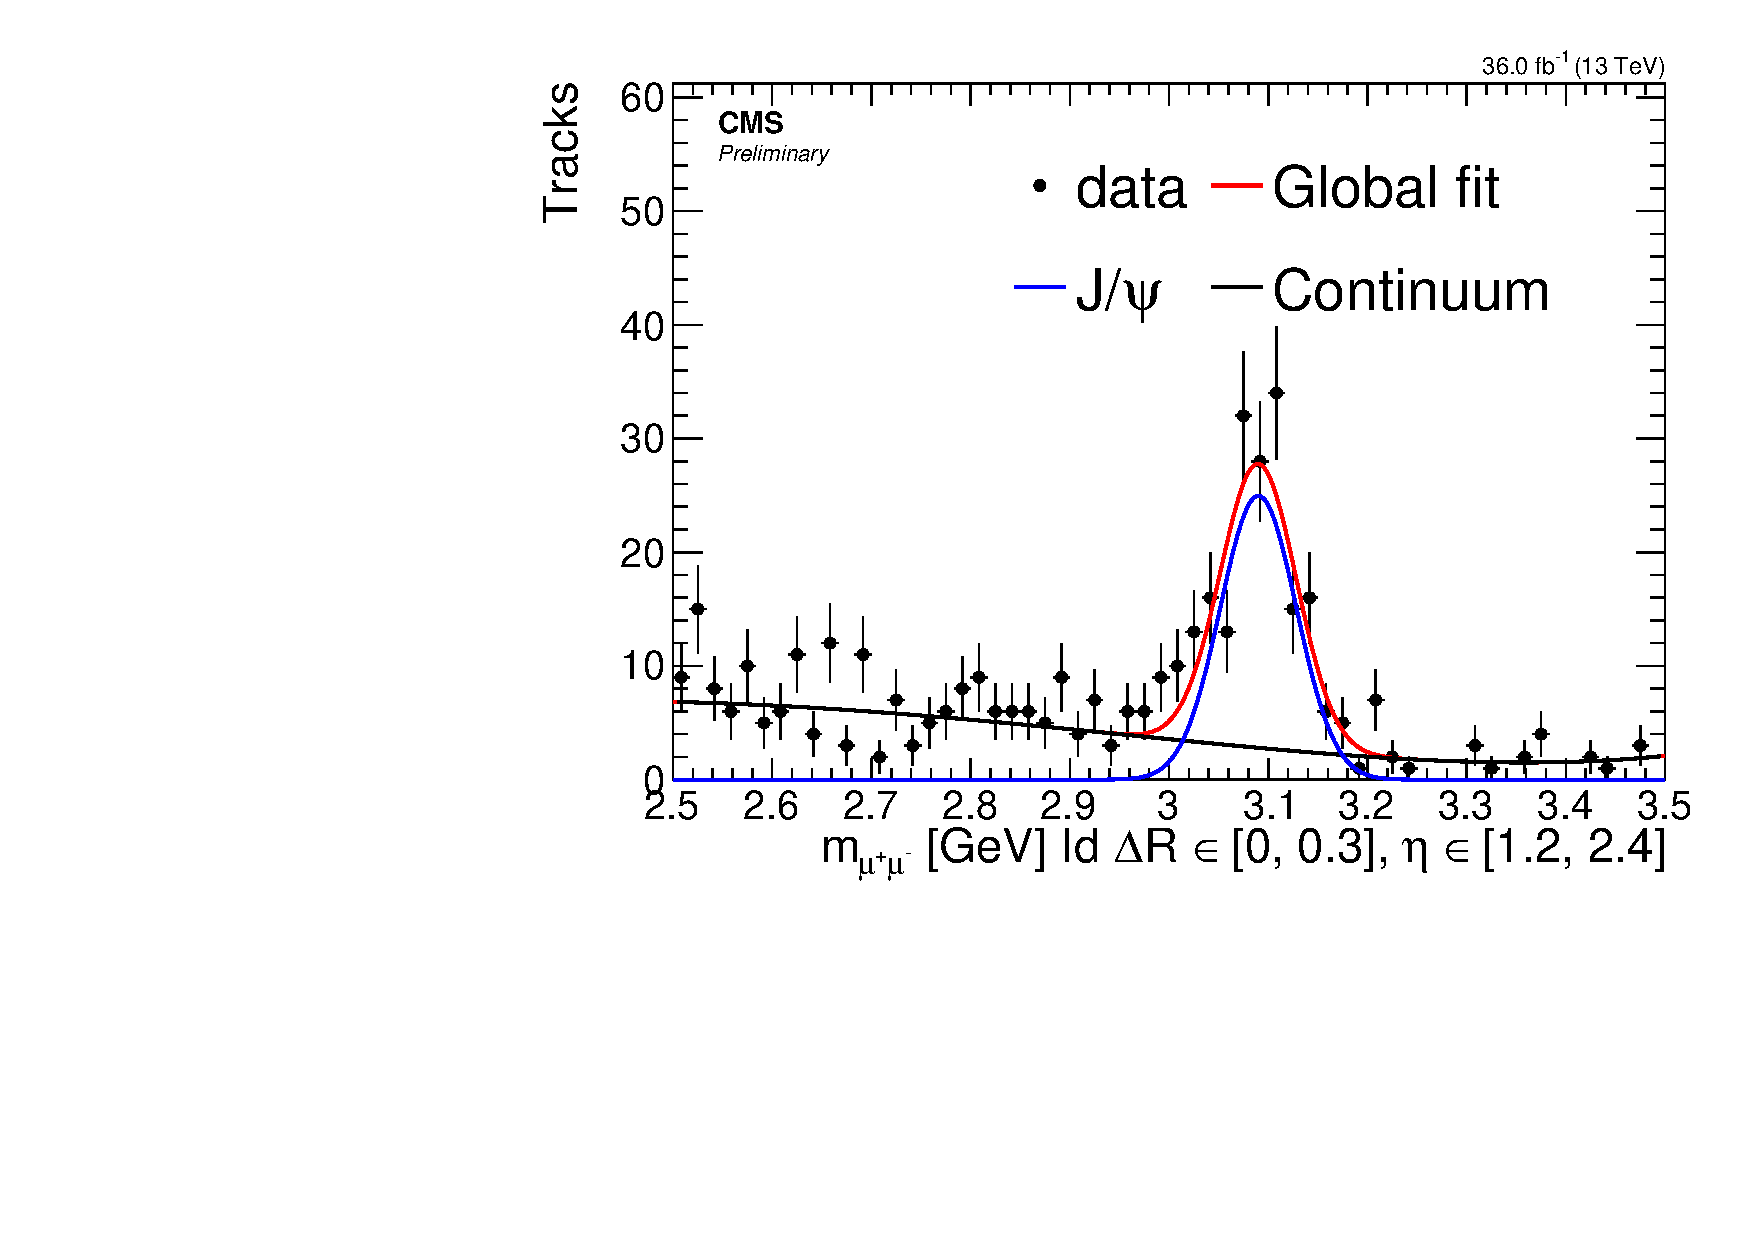
\includegraphics[width=0.32\linewidth]{plots/jpsi_muons_fit_data_delta_r_single_electron/none_id_invMass_0_0.3_1.2_2.4.pdf} \,
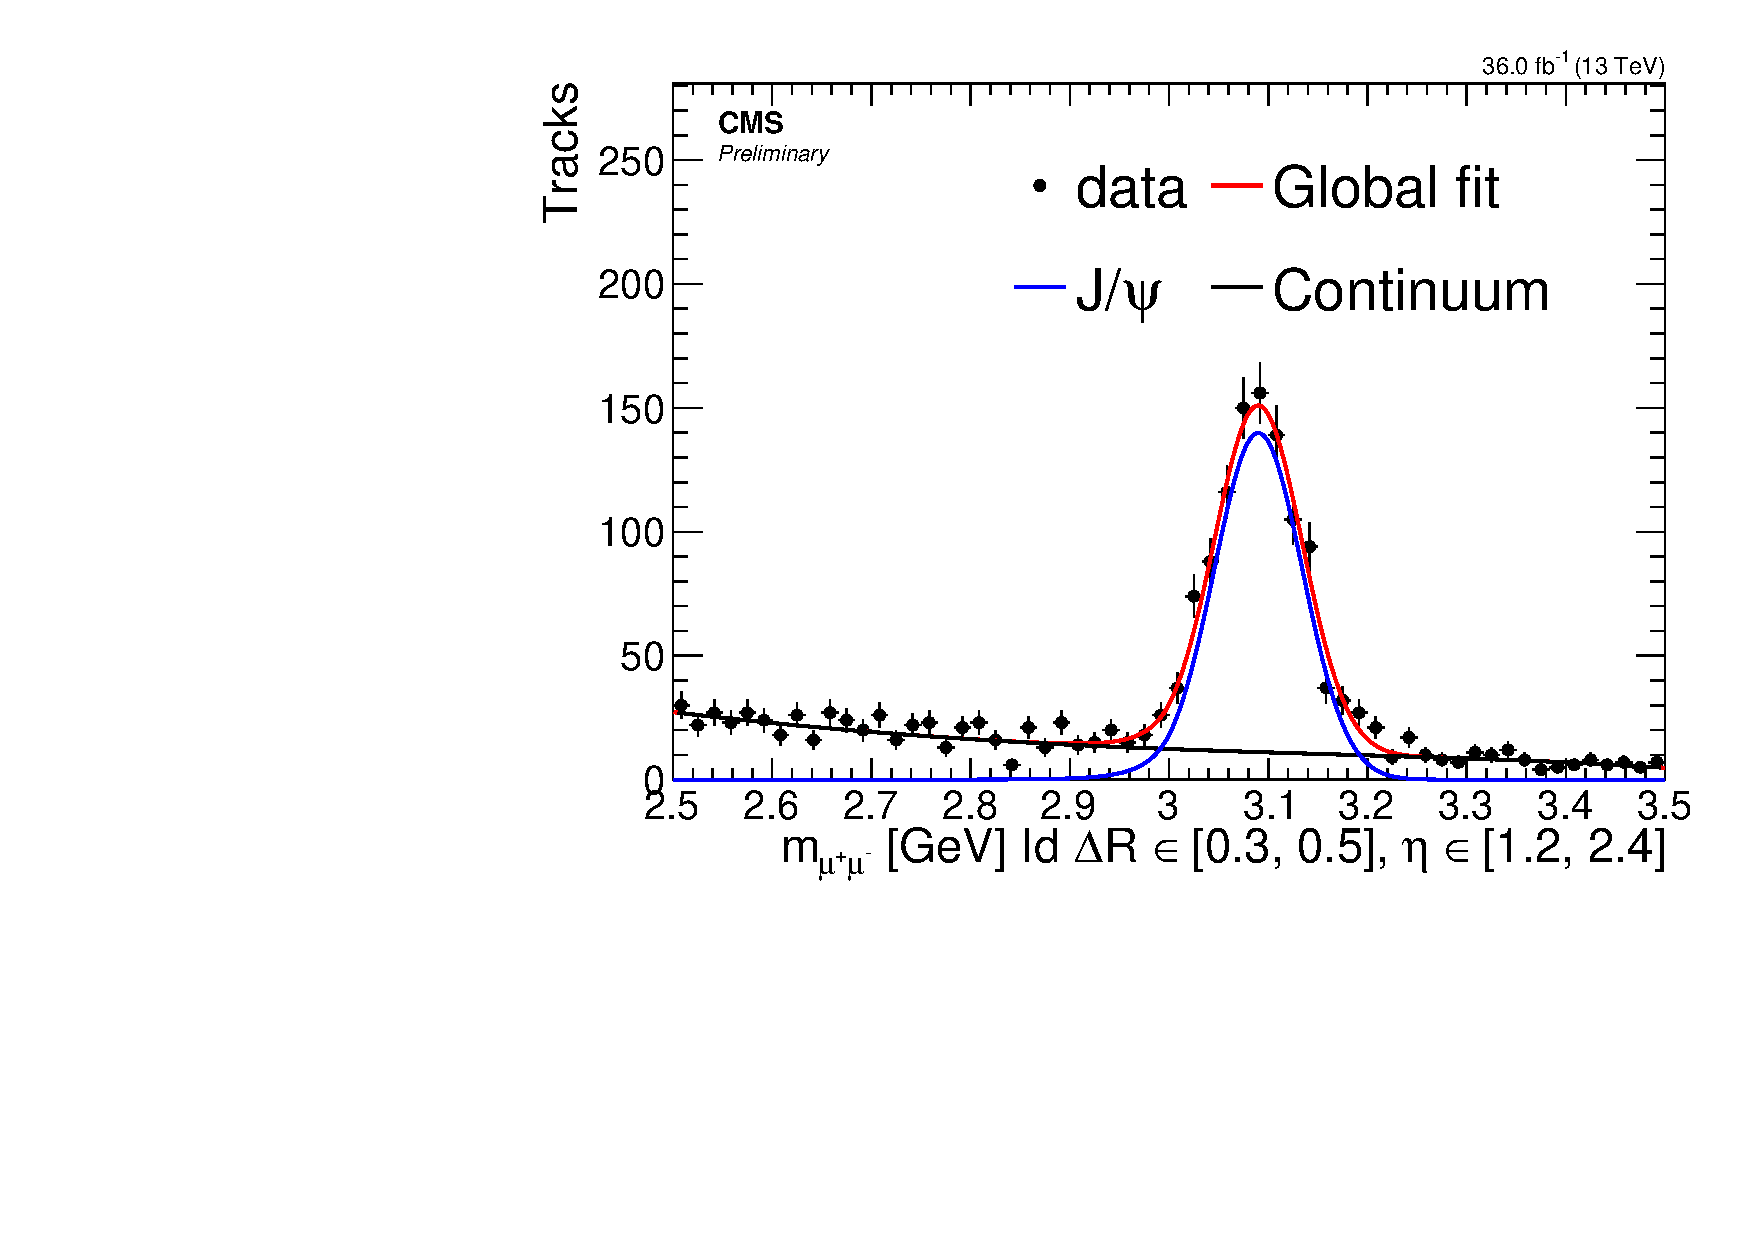
\includegraphics[width=0.32\linewidth]{plots/jpsi_muons_fit_data_delta_r_single_electron/none_id_invMass_0.3_0.5_1.2_2.4.pdf} \,
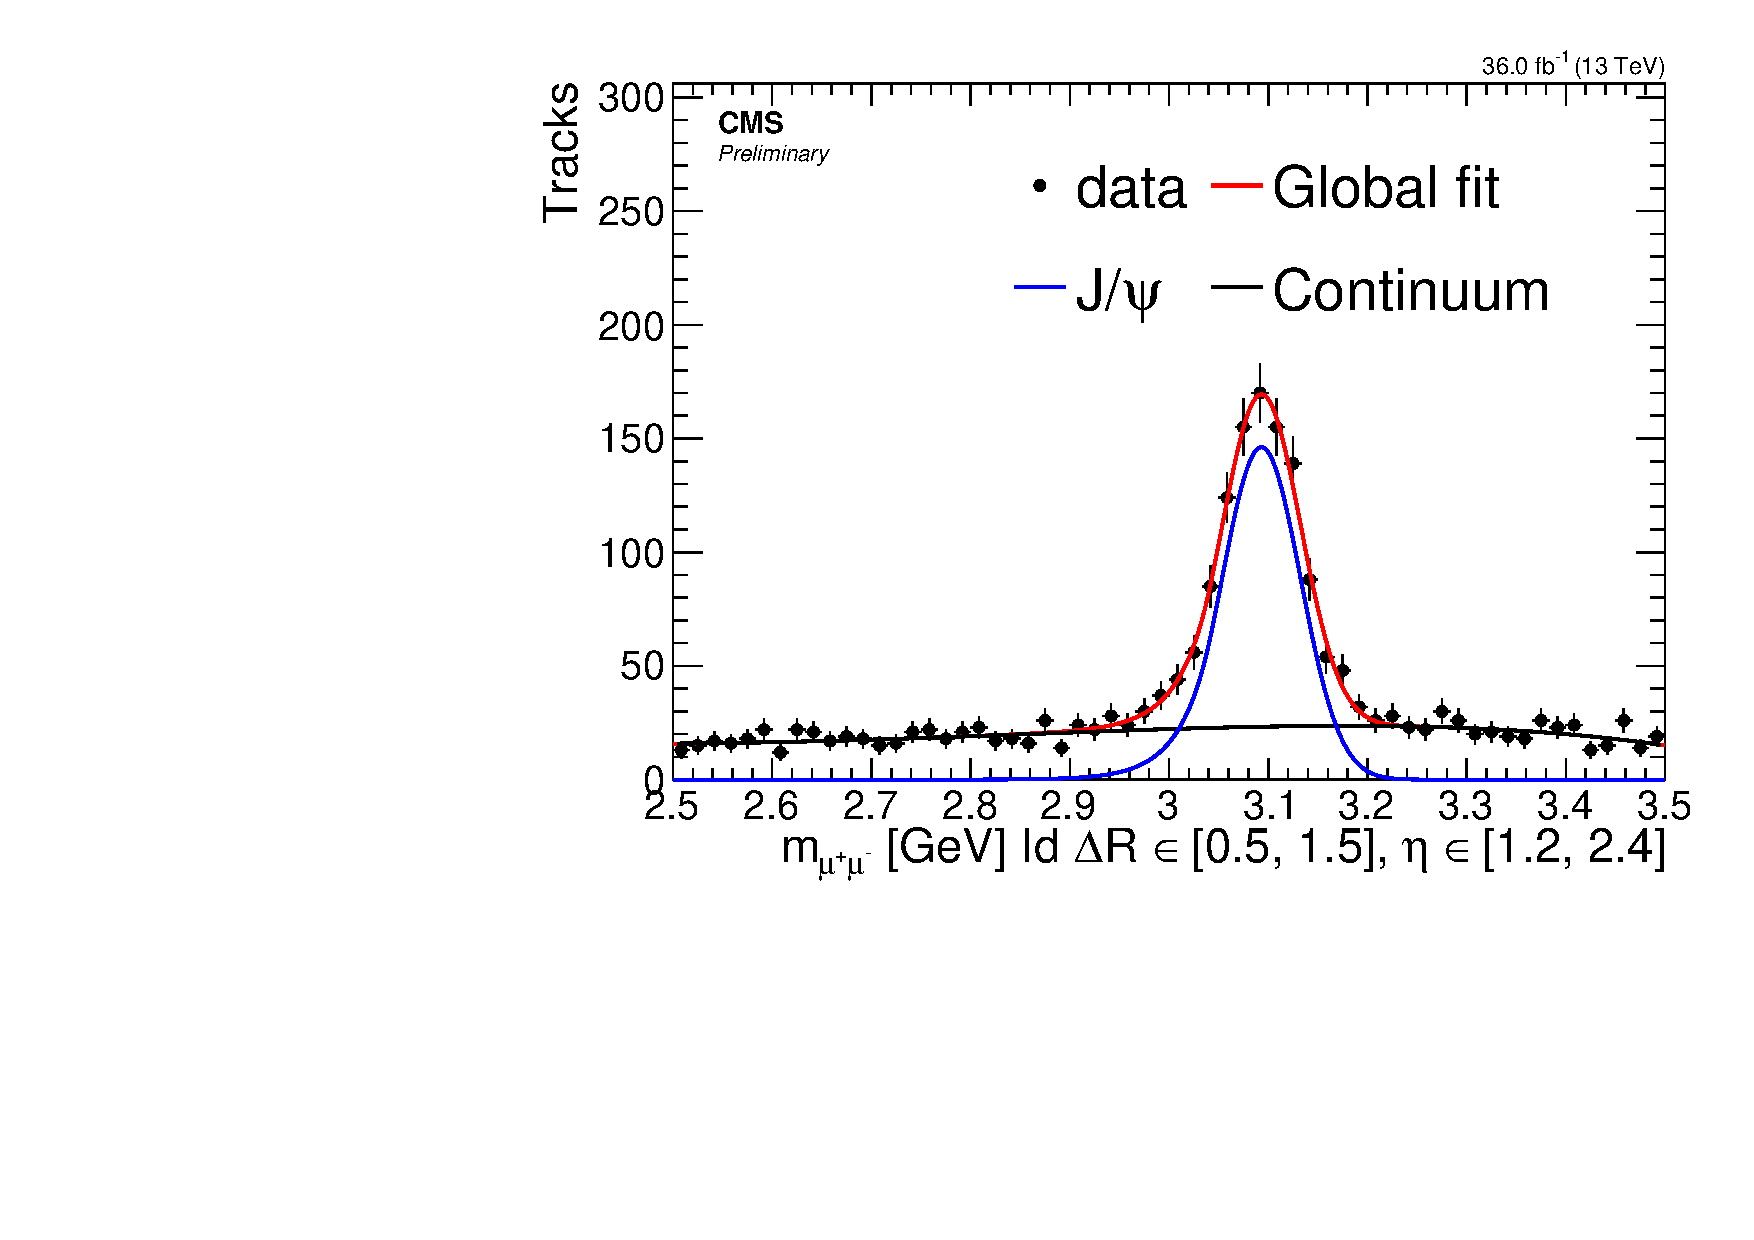
\includegraphics[width=0.32\linewidth]{plots/jpsi_muons_fit_data_delta_r_single_electron/none_id_invMass_0.5_1.5_1.2_2.4.pdf}  \\
\caption[Data endcaps muons fits]{Fits to the tag and probe invariant mass for muons in the endcaps region based on data. Results are shown for denominator (top) and numerator (bottom) for $0<\DR<0.3$  (left), $0.3<\DR<0.5$ (center), $0.5<\DR<1.5$ (right).}
\label{fig:tb-endcaps-data}
\end{figure}

The efficiency and corresponding scale factors are shown in Figure~\ref{fig:tb-eff-sf}. The scale factors are statistically consistent with unity and show no discernible $\DR$ dependence. A similar study was carried out based on 2017 and 2018 data and \gls{mc}~\cite{muon-id-sf-2017-8}, and no $\DR$ dependence was observed either. As a result of these studies, the recommendation from the \gls{pog} is to use the calculated scale factors provided by them with an additional systematic uncertainty of 1\% for muons with $\pt<20\GeV$.

\begin{figure}[!htbp]
\centering
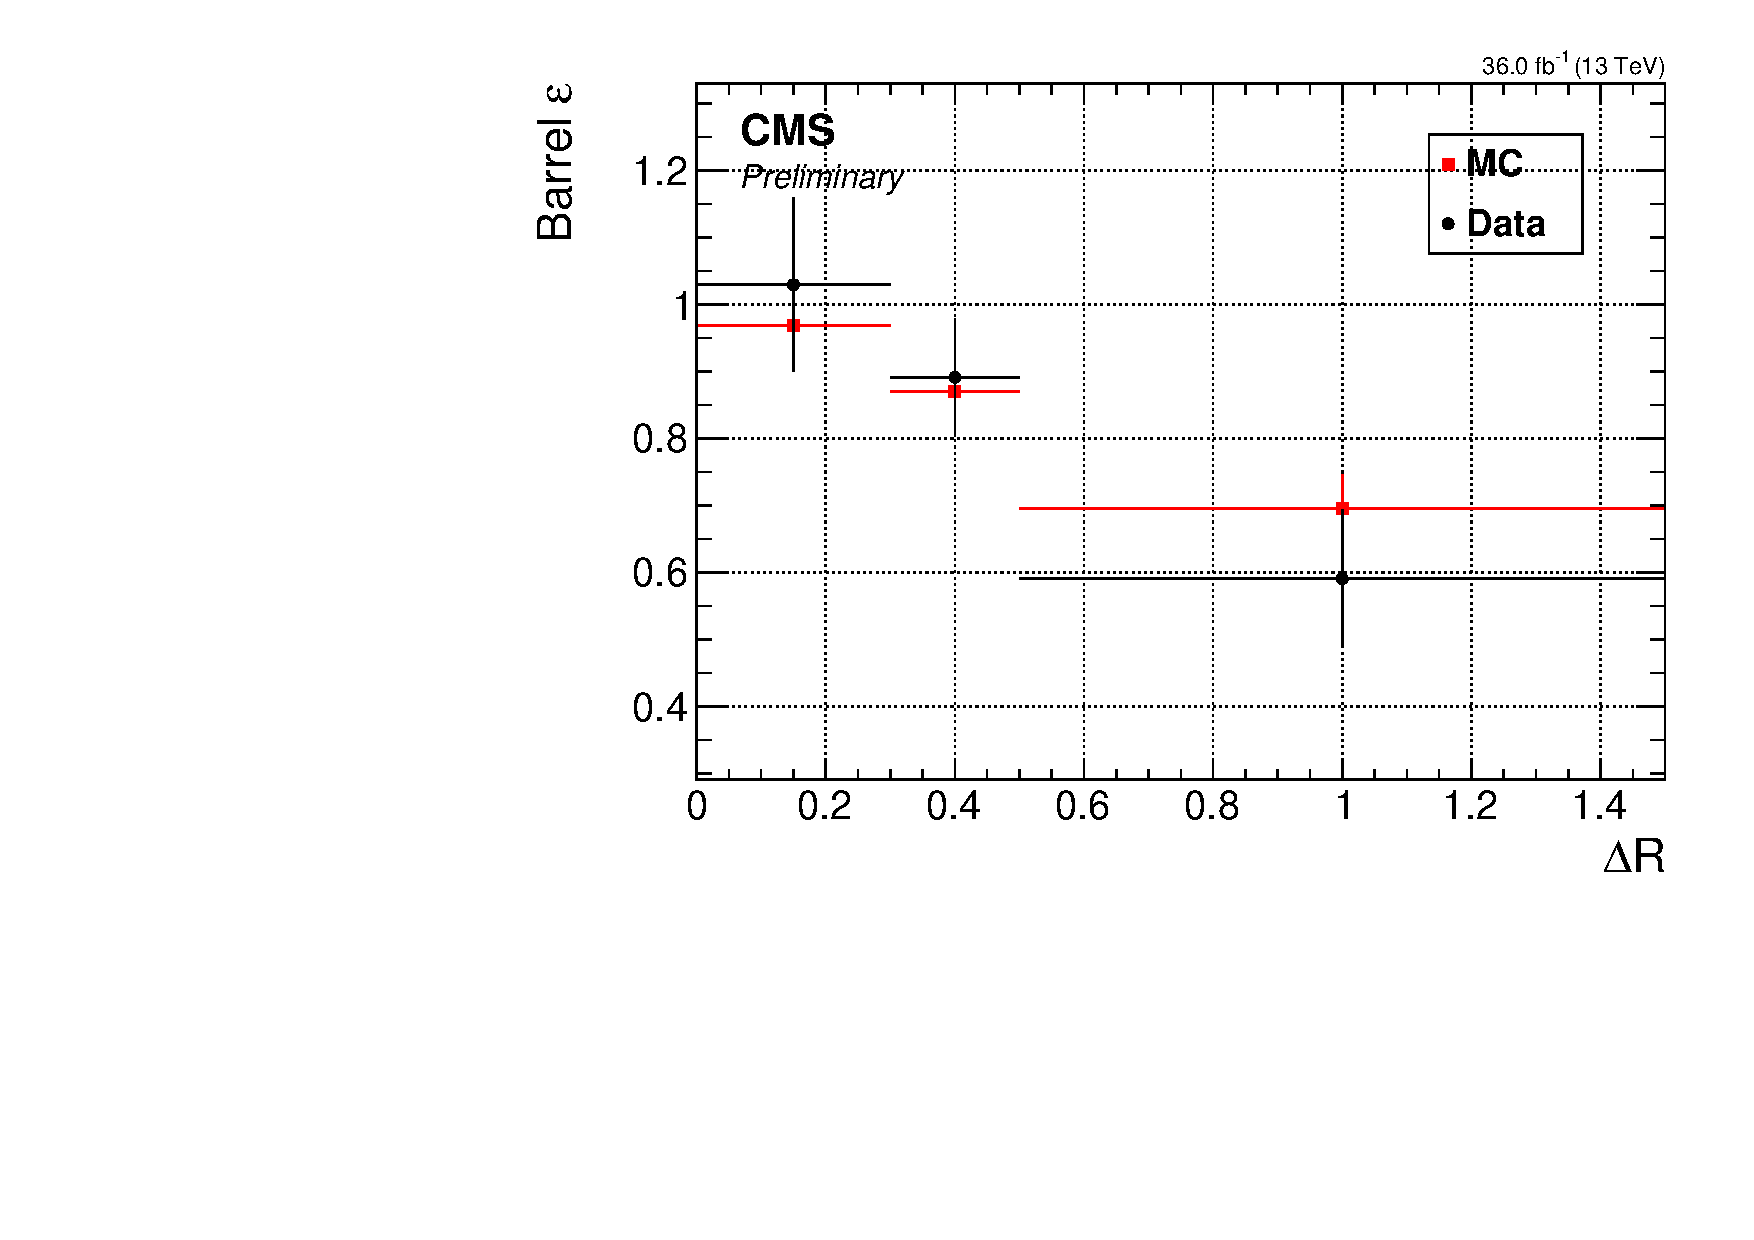
\includegraphics[width=0.48\linewidth]{plots/scale_factors/barrelDeltaRSingleElectron.pdf} \,
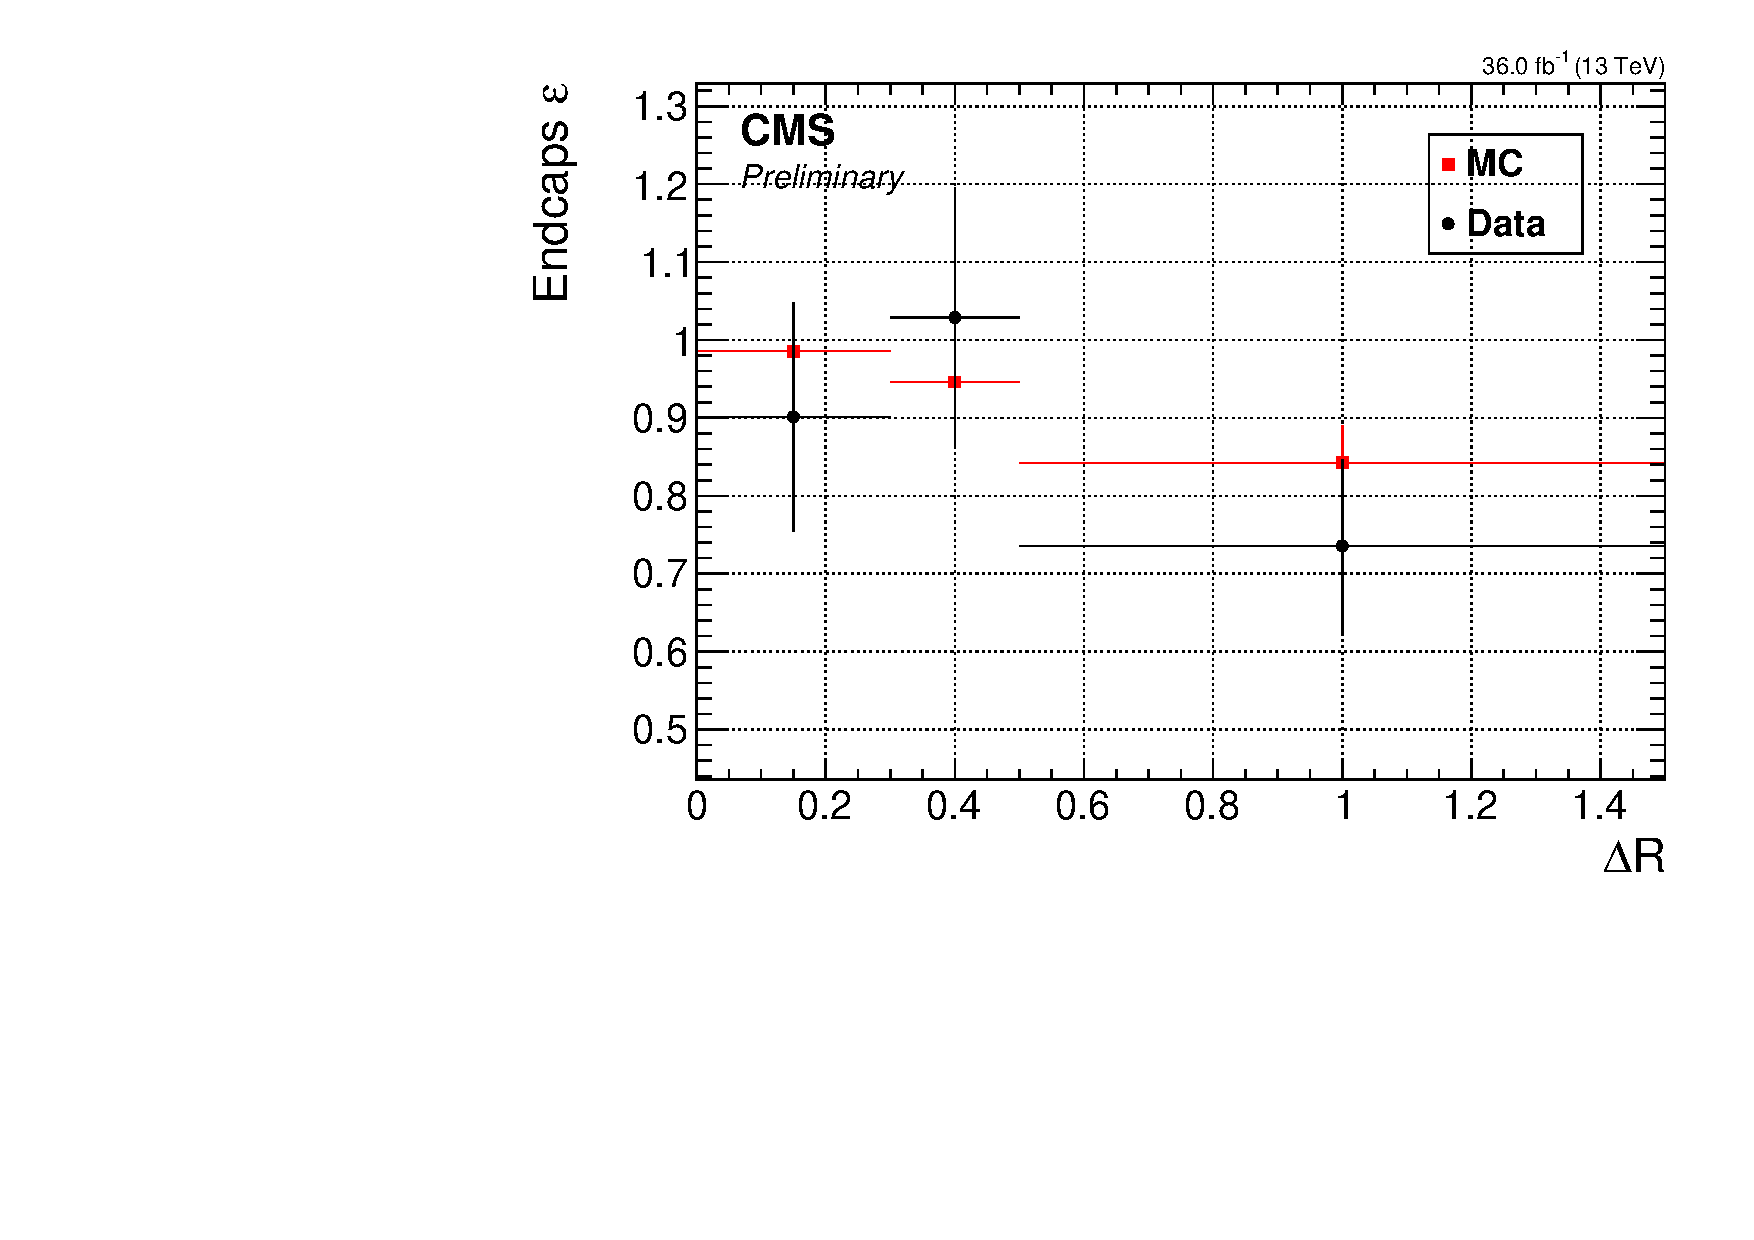
\includegraphics[width=0.48\linewidth]{plots/scale_factors/endcapsDeltaRSingleElectron.pdf}  \\
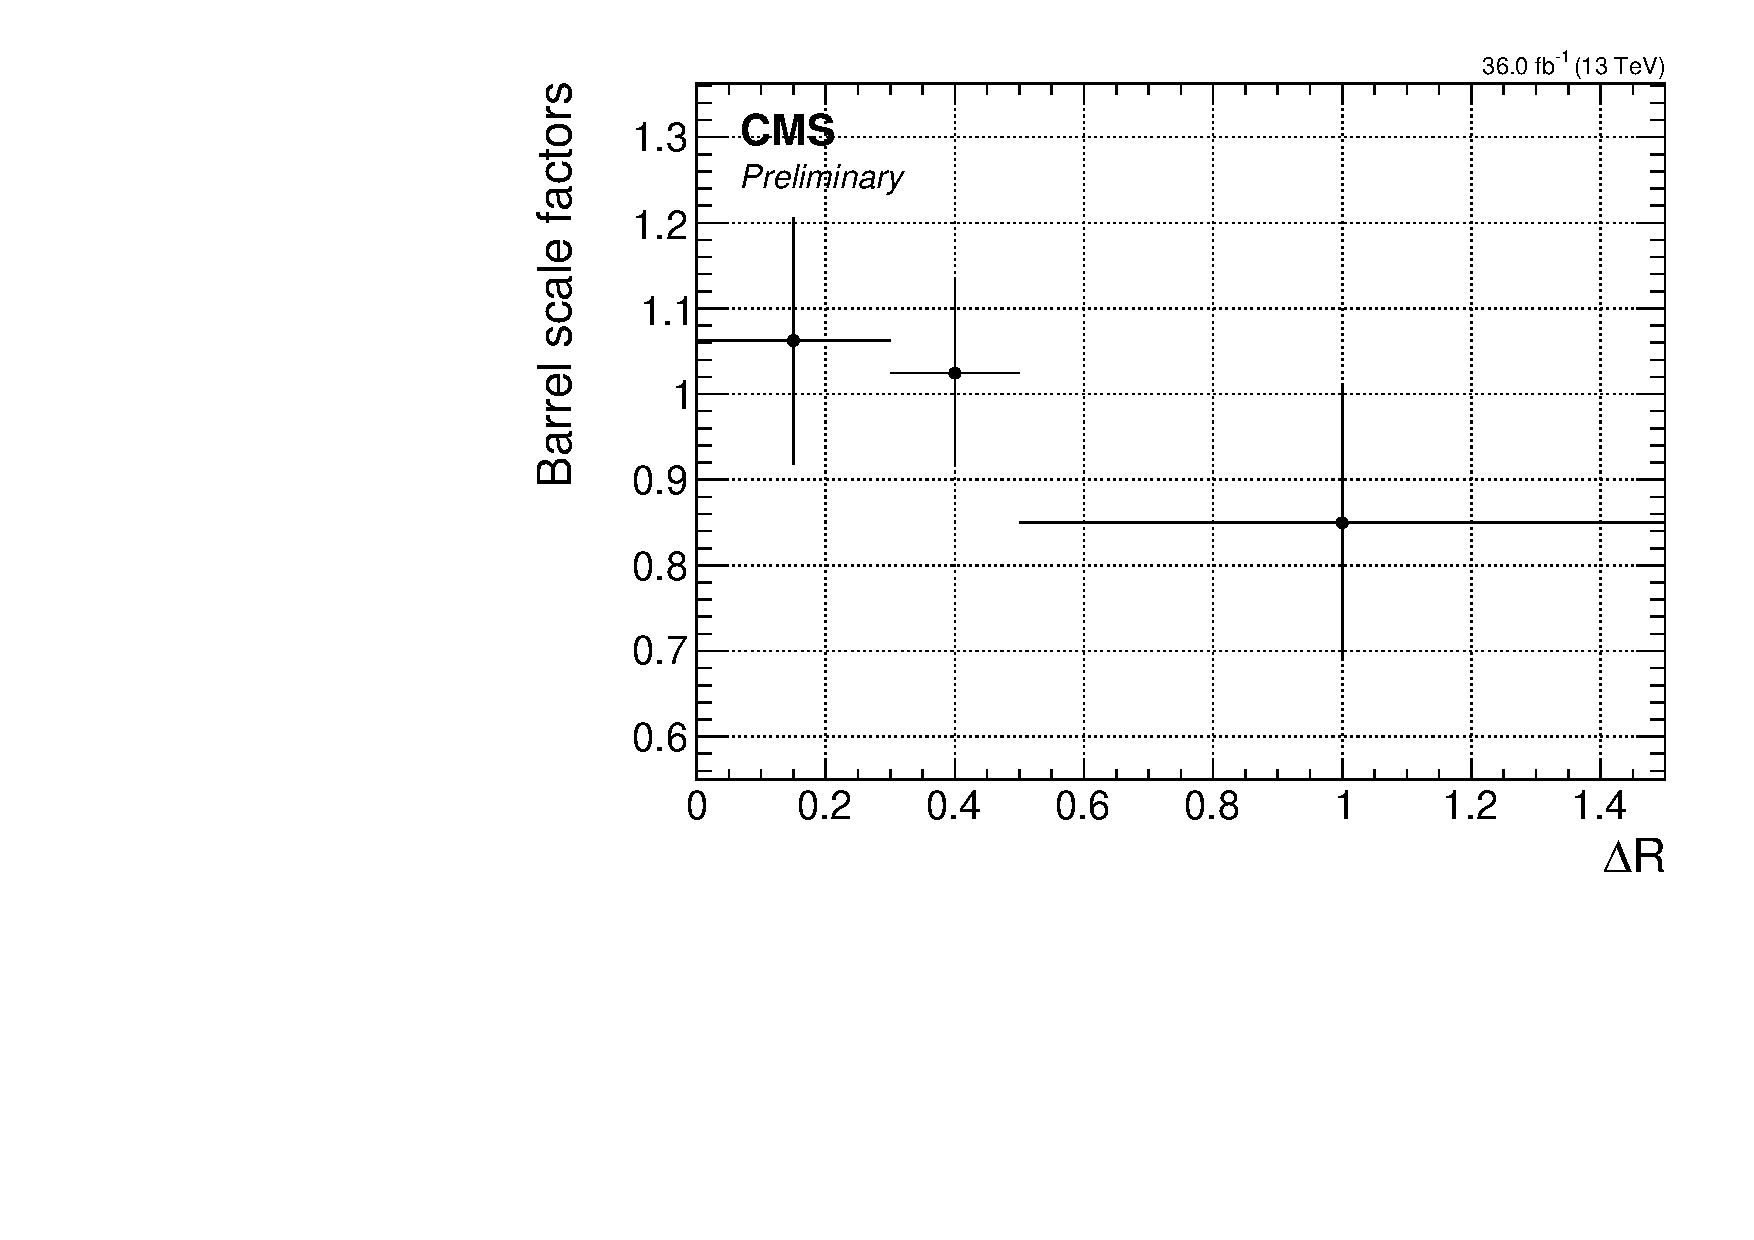
\includegraphics[width=0.48\linewidth]{plots/scale_factors/barrelDeltaRisoScaleFactorsSingleElectron.pdf} \,
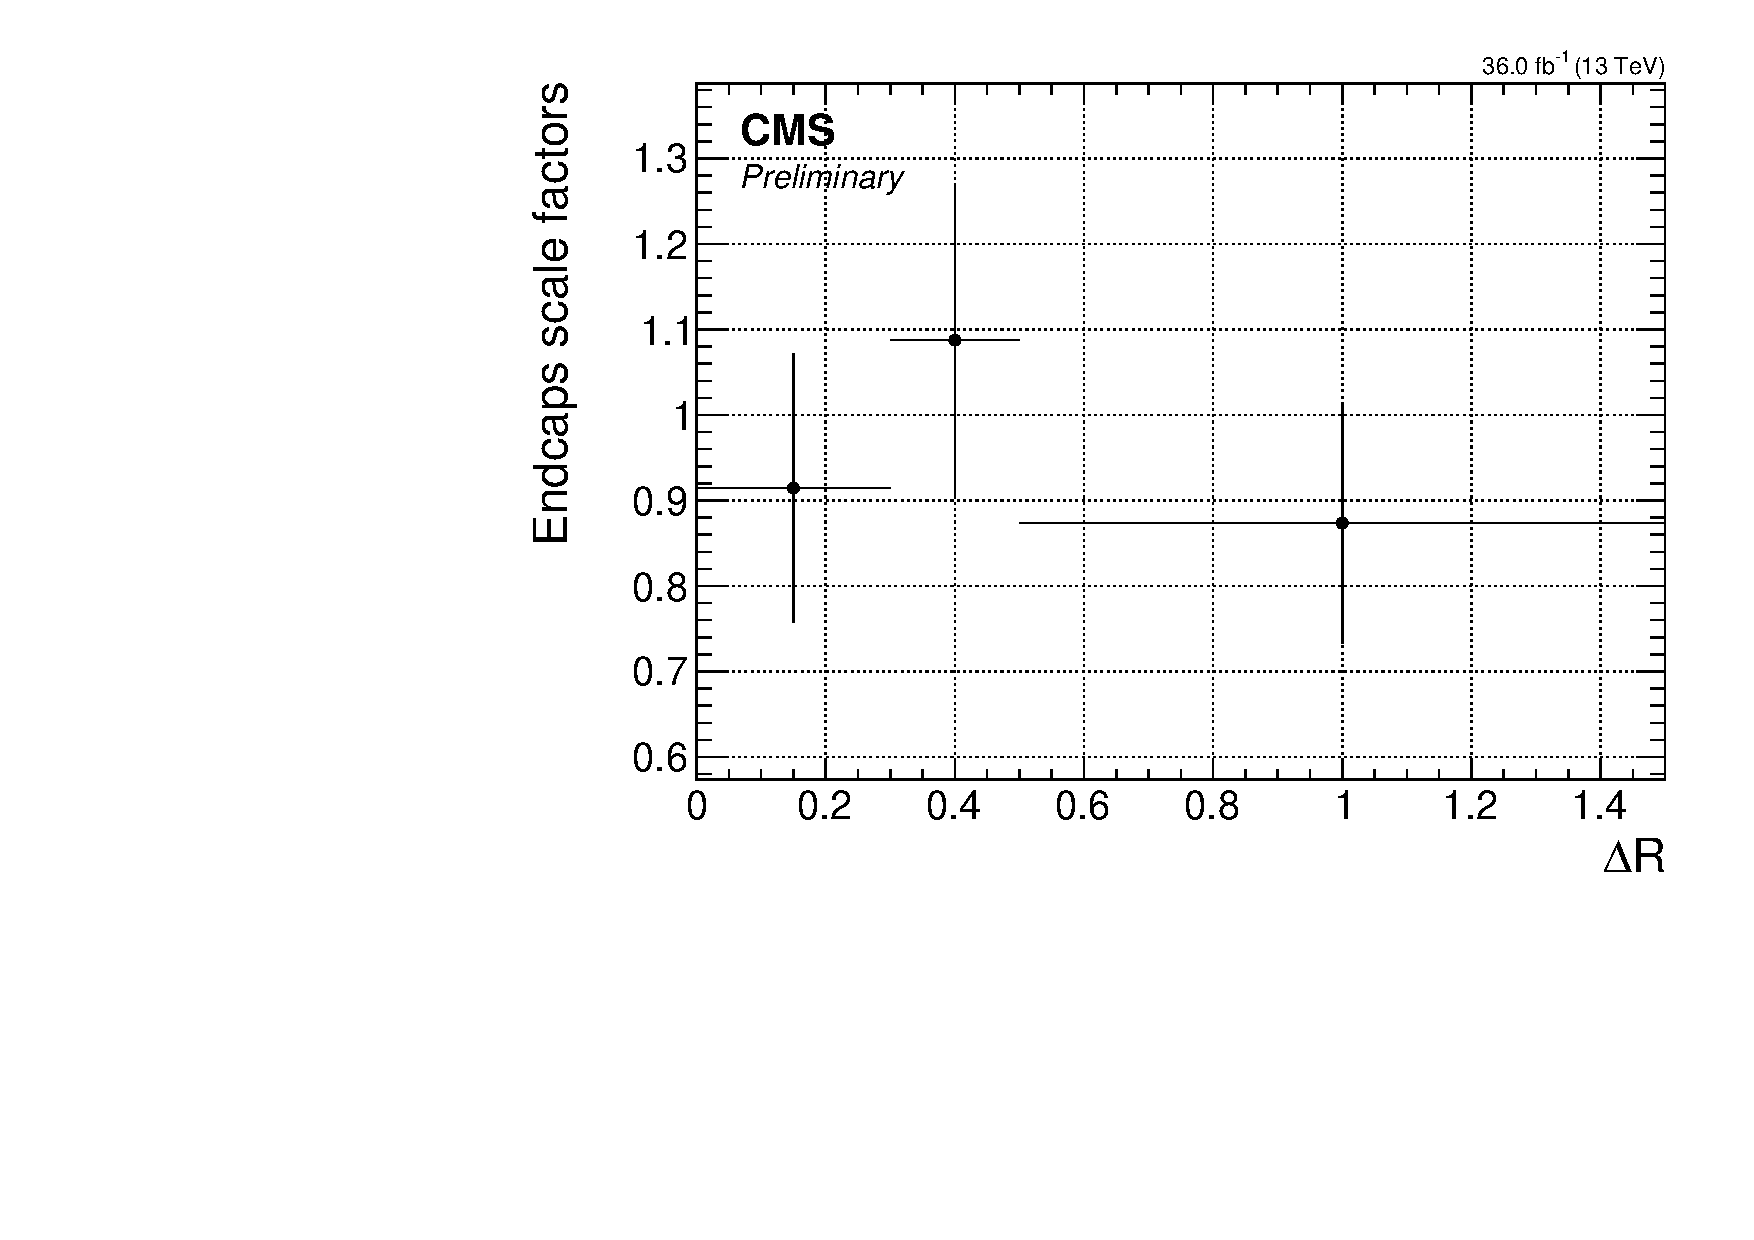
\includegraphics[width=0.48\linewidth]{plots/scale_factors/endcapsDeltaRisoScaleFactorsSingleElectron.pdf} \\
\caption[Efficienciy values and scale factors]{Efficiencies (top) and scale factors (bottom) for barrel muons (left) and endcaps muons (right).}
\label{fig:tb-eff-sf}
\end{figure}